\begin{enumerate}[label=\thechapter.\arabic*,ref=\thechapter.\theenumi]

\item The number of zeroes of the polynomial $P(s) = s^3+2s^2+5s+80$ in the right side of the plane?\hfill(GATE IN 2023) \\

\solution
\iffalse
\let\negmedspace\undefined
\let\negthickspace\undefined
\documentclass[journal,12pt,twocolumn]{IEEEtran}
\usepackage{cite}
\usepackage{amsmath,amssymb,amsfonts}
\usepackage{graphicx}
\usepackage{textcomp}
\usepackage{xcolor}
\usepackage{txfonts}
\usepackage{listings}
\usepackage{enumitem}
\usepackage{mathtools}
\usepackage{gensymb}
\usepackage{comment}
\usepackage[breaklinks=true]{hyperref}
\usepackage{tkz-euclide} 
\usepackage{listings}
\usepackage{gvv}                                        
\def\inputGnumericTable{}                                 
\usepackage[latin1]{inputenc}                                
\usepackage{color}                                            
\usepackage{array}                                            
\usepackage{longtable}                                       
\usepackage{calc}                                             
\usepackage{multirow}                                         
\usepackage{hhline}                                           
\usepackage{ifthen}                                           
\usepackage{lscape}
\usepackage[export]{adjustbox}

\newtheorem{theorem}{Theorem}[section]
\newtheorem{problem}{Problem}
\newtheorem{proposition}{Proposition}[section]
\newtheorem{lemma}{Lemma}[section]
\newtheorem{corollary}[theorem]{Corollary}
\newtheorem{example}{Example}[section]
\newtheorem{definition}[problem]{Definition}
\newcommand{\BEQA}{\begin{eqnarray}}
\newcommand{\EEQA}{\end{eqnarray}}
\newcommand{\define}{\stackrel{\triangle}{=}}
\newtheorem{rem}{Remark}

\begin{document}
\parindent 0px
\bibliographystyle{IEEEtran}

\vspace{3cm}

\title{}
\author{EE23BTECH11042 -  Khusinadha Naik$^{*}$
}
\maketitle
\newpage
\bigskip

% \renewcommand{\thefigure}{\theenumi}
% \renewcommand{\thetable}{\theenumi}


\noindent \textbf{26.} \hspace{2pt}A causal, discrete time system is described by the difference equation $y[n] = 0.5 y[n-1] + x[n]$, for all $n$, where $y[n]$ denotes the output sequence and $x[n]$ denotes the input sequence. Which of the following statements is/are TRUE?
\begin{flushright}
\hfill(GATE 2023 BM)
\end{flushright}
\begin{enumerate}[label = (\alph*)]
	\item The system has an impulse response described by $0.5^{n} u[-n]$ where $u[n]$ is the  
unit step sequence. 	\label{option:GATE.2023.BM.26.1}	
	\item The system is stable in the bounded input, bounded output sense.		\label{option:GATE.2023.BM.26.2}
	\item The system has an infinite number of non-zero samples in its impulse response	\label{option:GATE.2023.BM.26.3}
	\item The system has a finite number of non-zero samples in its impulse response.	\label{option:GATE.2023.BM.26.4}
\end{enumerate}

\noindent \textbf{Ans.}\\
\fi
\begin{table}[h]
\centering
\begin{tabular}{|c|c|c|}
        \hline
        \textbf{Parameter} & \textbf{Value} & \textbf{Description} \\
        \hline
        $x[n]$ & ? & Input Sequence \\
        \hline
        $y[n]$ & ? & Output Sequence \\
        \hline
\end{tabular}
\caption{Input parameters table}
\label{tab:GATE.2023.BM.26.1}





\end{table}
\begin{align}
y[n] = 0.5y[n-1] + x[n] 
\end{align}

Taking $Z$-Transform 
\begin{align}
Y\brak{z} &= 0.5z^{-1}Y\brak{z} + X\brak{z} \\
\implies \frac{Y\brak{z}}{X\brak{z}} &= \frac{1}{1 - 0.5z^{-1}} = H\brak{z} 
\end{align}
If $x[n]$ is impulse input 
\begin{align}
\implies &Y\brak{z} = H\brak{z} = \frac{1}{1 - 0.5z^{-1}}  \label{eq:GATE.2023.BM.26.4}
\end{align}
From \eqref{eq:GATE.2023.BM.26.4} pole lies at $z = 0.5$
\begin{align}
a^{n}u\brak{n} \xleftrightarrow{\mathcal{Z}} &\frac{1}{1 - az^{-1}} \quad , \abs{z} > a \label{eq:GATE.2023.BM.26.5}
\end{align}

From \eqref{eq:GATE.2023.BM.26.4} , \eqref{eq:GATE.2023.BM.26.5}
\begin{align}
h[n] = 0.5^{n}u[n] \quad , \abs{z} > 0.5 \label{eq:GATE.2023.BM.26.6}
\end{align}


\pagebreak
Plotting $h[n]$ vs $n$
\begin{figure}[h]
    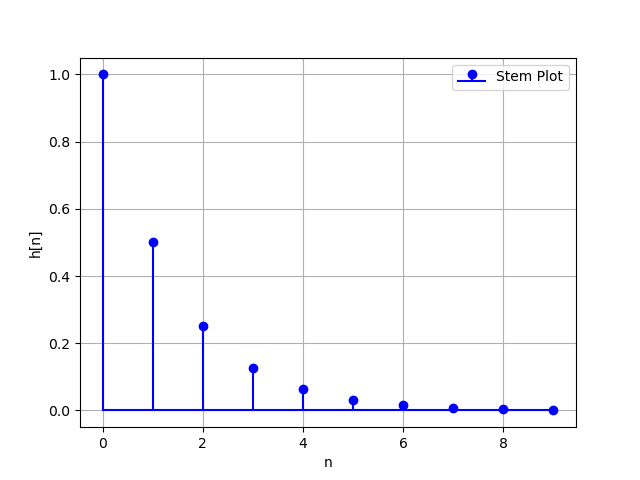
\includegraphics[width=0.5\textwidth]{2023/BM/26/figs/fig1.png}
    \caption{Plot of $h[n]$ vs $n$}
    \label{fig:GATE.2023.BM.26.1}
\end{figure}

\begin{enumerate}
\item From \eqref{eq:GATE.2023.BM.26.6} , \ref{option:GATE.2023.BM.26.1} is wrong
\item As pole lies within unit circle \ref{option:GATE.2023.BM.26.2} is true
\item From \eqref{eq:GATE.2023.BM.26.6} and \figref{fig:GATE.2023.BM.26.1} ,\ref{option:GATE.2023.BM.26.3} is true and hence
\item \ref{option:GATE.2023.BM.26.4} is false 
\end{enumerate}





%\end{document}

\newpage

\item The circuit shown in the figure is initially in the steady state with the switch K in open condition and $\overline{K}$ in closed condition. The switch K is closed and $\overline{K}$ is opened simultaneously at the instant $t = t_1$, where $t_1 > 0$. The minimum value of $t_1$ in milliseconds such that there is no transient in the voltage across the 100 $\mu F$ capacitor, is \rule{1cm}{0.15mm} (Round off to 2 decimal places) \hfill (GATE EE 2023)
\begin{circuitikz}
     \draw (0,0) node[left] {$x_1(t)$} to (0.8,0);
     \draw (0,-1) node[left] {$x_2(t)$} to (0.8,-1);
     \draw (1,0) circle(0.2);
     \draw (1,0) node {$\times$};
     \draw (1,-1) circle(0.2);
     \draw (1,-1) node {$\times$};
    \draw (1.2,0) to (1.8,0);
    \draw (1.2,-1) to (1.8,-1);
    \draw (1.8,0) to (1.8,-0.3);
    \draw (1.8,-1) to (1.8,-0.7);
    \draw (1.8,-0.5) circle(0.2);
    \draw (1.8,-0.5) node {$+$};
    \draw[->] (1,0.5) to (1,0.2) ;
    \node at (1,0.6) {cos$(4\pi\times10^3t)$};
    \draw[->] (1,-1.5) to (1,-1.2);
    \node at (1,-1.6) {cos$(12\pi\times10^3t)$};
    \draw (2,-0.5) to (2.3,-0.5);
    \node at (2.6,-0.5) {y(t)};
     
     
\end{circuitikz}
\\
\solution
\iffalse
\let\negmedspace\undefined
\let\negthickspace\undefined
\documentclass[journal,12pt,twocolumn]{IEEEtran}
\usepackage{cite}
\usepackage{amsmath,amssymb,amsfonts}
\usepackage{graphicx}
\usepackage{textcomp}
\usepackage{xcolor}
\usepackage{txfonts}
\usepackage{listings}
\usepackage{enumitem}
\usepackage{mathtools}
\usepackage{gensymb}
\usepackage{comment}
\usepackage[breaklinks=true]{hyperref}
\usepackage{tkz-euclide} 
\usepackage{listings}
\usepackage{gvv}                                        
\def\inputGnumericTable{}                                 
\usepackage[latin1]{inputenc}                                
\usepackage{color}                                            
\usepackage{array}                                            
\usepackage{longtable}                                       
\usepackage{calc}                                             
\usepackage{multirow}                                         
\usepackage{hhline}                                           
\usepackage{ifthen}                                           
\usepackage{lscape}
\usepackage[export]{adjustbox}

\newtheorem{theorem}{Theorem}[section]
\newtheorem{problem}{Problem}
\newtheorem{proposition}{Proposition}[section]
\newtheorem{lemma}{Lemma}[section]
\newtheorem{corollary}[theorem]{Corollary}
\newtheorem{example}{Example}[section]
\newtheorem{definition}[problem]{Definition}
\newcommand{\BEQA}{\begin{eqnarray}}
\newcommand{\EEQA}{\end{eqnarray}}
\newcommand{\define}{\stackrel{\triangle}{=}}
\newtheorem{rem}{Remark}

\begin{document}
\parindent 0px
\bibliographystyle{IEEEtran}

\vspace{3cm}

\title{}
\author{EE23BTECH11042 -  Khusinadha Naik$^{*}$
}
\maketitle
\newpage
\bigskip

% \renewcommand{\thefigure}{\theenumi}
% \renewcommand{\thetable}{\theenumi}


\noindent \textbf{26.} \hspace{2pt}A causal, discrete time system is described by the difference equation $y[n] = 0.5 y[n-1] + x[n]$, for all $n$, where $y[n]$ denotes the output sequence and $x[n]$ denotes the input sequence. Which of the following statements is/are TRUE?
\begin{flushright}
\hfill(GATE 2023 BM)
\end{flushright}
\begin{enumerate}[label = (\alph*)]
	\item The system has an impulse response described by $0.5^{n} u[-n]$ where $u[n]$ is the  
unit step sequence. 	\label{option:GATE.2023.BM.26.1}	
	\item The system is stable in the bounded input, bounded output sense.		\label{option:GATE.2023.BM.26.2}
	\item The system has an infinite number of non-zero samples in its impulse response	\label{option:GATE.2023.BM.26.3}
	\item The system has a finite number of non-zero samples in its impulse response.	\label{option:GATE.2023.BM.26.4}
\end{enumerate}

\noindent \textbf{Ans.}\\
\fi
\begin{table}[h]
\centering
\begin{tabular}{|c|c|c|}
        \hline
        \textbf{Parameter} & \textbf{Value} & \textbf{Description} \\
        \hline
        $x[n]$ & ? & Input Sequence \\
        \hline
        $y[n]$ & ? & Output Sequence \\
        \hline
\end{tabular}
\caption{Input parameters table}
\label{tab:GATE.2023.BM.26.1}





\end{table}
\begin{align}
y[n] = 0.5y[n-1] + x[n] 
\end{align}

Taking $Z$-Transform 
\begin{align}
Y\brak{z} &= 0.5z^{-1}Y\brak{z} + X\brak{z} \\
\implies \frac{Y\brak{z}}{X\brak{z}} &= \frac{1}{1 - 0.5z^{-1}} = H\brak{z} 
\end{align}
If $x[n]$ is impulse input 
\begin{align}
\implies &Y\brak{z} = H\brak{z} = \frac{1}{1 - 0.5z^{-1}}  \label{eq:GATE.2023.BM.26.4}
\end{align}
From \eqref{eq:GATE.2023.BM.26.4} pole lies at $z = 0.5$
\begin{align}
a^{n}u\brak{n} \xleftrightarrow{\mathcal{Z}} &\frac{1}{1 - az^{-1}} \quad , \abs{z} > a \label{eq:GATE.2023.BM.26.5}
\end{align}

From \eqref{eq:GATE.2023.BM.26.4} , \eqref{eq:GATE.2023.BM.26.5}
\begin{align}
h[n] = 0.5^{n}u[n] \quad , \abs{z} > 0.5 \label{eq:GATE.2023.BM.26.6}
\end{align}


\pagebreak
Plotting $h[n]$ vs $n$
\begin{figure}[h]
    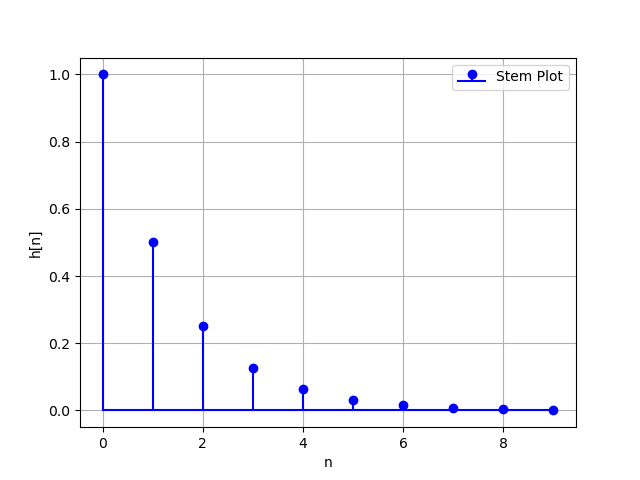
\includegraphics[width=0.5\textwidth]{2023/BM/26/figs/fig1.png}
    \caption{Plot of $h[n]$ vs $n$}
    \label{fig:GATE.2023.BM.26.1}
\end{figure}

\begin{enumerate}
\item From \eqref{eq:GATE.2023.BM.26.6} , \ref{option:GATE.2023.BM.26.1} is wrong
\item As pole lies within unit circle \ref{option:GATE.2023.BM.26.2} is true
\item From \eqref{eq:GATE.2023.BM.26.6} and \figref{fig:GATE.2023.BM.26.1} ,\ref{option:GATE.2023.BM.26.3} is true and hence
\item \ref{option:GATE.2023.BM.26.4} is false 
\end{enumerate}





%\end{document}


\newpage
\item $y=e^{mx}+e^{-mx}$ is the solution of which differential equation?
\begin{enumerate}[label=\textbf{\arabic*.}, font=\bfseries, align=left]
    \item $\frac{dy}{dx} - my = 0$ 
    \item $\frac{dy}{dx} + my = 0$ 
    \item $\frac{d^{2}y}{dx^{2}} + m^{2}y = 0$ 
    \item $\frac{d^{2}y}{dx^{2}} - m^{2}y = 0$ 
\end{enumerate} \hfill(GATE AG 2023)
\solution

\newpage
\item  A cascade control strategy is shown in the figure below. The transfer function between the output $(y)$ and the secondary disturbance $(d_2)$ is defined as  \\
$$G_{d2}(s)= \frac{y(s)}{d_2(s)}$$. 
Which one of the following is the CORRECT expression for the transfer function $G_{d2}(s)$? \\
\begin{figure}[h]
    \centering
    \includegraphics[scale=0.25]{2023/CH/44/figs/g44fig1.jpeg}
    \caption{ }
    \label{}
\end{figure}
\begin{enumerate}[label=\Alph*.]
\item $\frac{1}{(11s+21)(0.1s+1)}$ 
\item $\frac{1}{(s+1)(0.1s+1)}$
\item $\frac{(s+1)}{(s+2)(0.1s+1)}$
\item $\frac{(s+1)}{(s+1)(0.1s+1)}$
\end{enumerate} \hfill (GATE CH 2023)
\solution
\input{2023/CH/44/g44.1.tex}
\newpage
\item In the differential equation $\frac{dy}{dx} + \alpha x y = 0, \alpha$ is a positive constant. If $y = 1.0$ at
$x = 0.0$, and $y = 0.8$ at $x = 1.0$, the value of $\alpha$ is (rounded off to three decimal places).  \hfill(GATE CE 2023)
\solution

\newpage
\item The switch $S_1$ was closed and $S_2$ was open for a long time. At t=0,switch $S_1$ is opened and $S_2$ is closed,simultaneously. The value of $i_c(0^{+})$, in amperes, is  \hfill (GATE EC 44)\\
\begin{circuitikz}
     \draw (0,0) node[left] {$x_1(t)$} to (0.8,0);
     \draw (0,-1) node[left] {$x_2(t)$} to (0.8,-1);
     \draw (1,0) circle(0.2);
     \draw (1,0) node {$\times$};
     \draw (1,-1) circle(0.2);
     \draw (1,-1) node {$\times$};
    \draw (1.2,0) to (1.8,0);
    \draw (1.2,-1) to (1.8,-1);
    \draw (1.8,0) to (1.8,-0.3);
    \draw (1.8,-1) to (1.8,-0.7);
    \draw (1.8,-0.5) circle(0.2);
    \draw (1.8,-0.5) node {$+$};
    \draw[->] (1,0.5) to (1,0.2) ;
    \node at (1,0.6) {cos$(4\pi\times10^3t)$};
    \draw[->] (1,-1.5) to (1,-1.2);
    \node at (1,-1.6) {cos$(12\pi\times10^3t)$};
    \draw (2,-0.5) to (2.3,-0.5);
    \node at (2.6,-0.5) {y(t)};
     
     
\end{circuitikz}
\\
\solution \\
\documentclass[journal,12pt,twocolumn]{IEEEtran}

% Packages
\usepackage{cite}
\usepackage{amsmath,amssymb,amsfonts,amsthm}
\usepackage{graphicx}
\usepackage{textcomp}
\usepackage{xcolor}
\usepackage{txfonts}
\usepackage{listings}
\usepackage{enumitem}
\usepackage{mathtools}
\usepackage{float}
\usepackage{gensymb}
\usepackage{comment}
\usepackage{hyperref}
\usepackage{tkz-euclide}
\usepackage{gvv}
\usepackage[latin1]{inputenc}
\usepackage{color}
\usepackage{array}
\usepackage{longtable}
\usepackage{calc}
\usepackage{multirow}
\usepackage{hhline}
\usepackage{ifthen}
\usepackage{lscape}
\usepackage{subcaption}
\usepackage{tikz}
\usepackage{circuitikz}
\usepackage{wrapfig}
\usepackage{lipsum}
\usepackage[export]{adjustbox}
\usepackage{inputenc}

% Custom commands and macros
\newtheorem{theorem}{Theorem}[section]
\newtheorem{problem}{Problem}
\newtheorem{proposition}{Proposition}[section]
\newtheorem{lemma}{Lemma}[section]
\newtheorem{corollary}[theorem]{Corollary}
\newtheorem{example}{Example}[section]
\newtheorem{definition}[problem]{Definition}
\newtheorem{rem}{Remark}
\newcommand{\BEQA}{\begin{eqnarray}}
\newcommand{\EEQA}{\end{eqnarray}}
\newcommand{\define}{\stackrel{\triangle}{=}}
\renewcommand{\thefigure}{\theenumi}
\renewcommand{\thetable}{\theenumi}



\begin{document}

\title{GATE 2023 EC 49}
\author{EE23BTECH11045 - Palavelli Srija$^{*}$}
\maketitle

\bigskip

\textbf{Question 12.7.7:} 
Let $x(t) = 10 \cos(10.5 \omega t)$ be passed through an LTI system with impulse response $h(t) = \pi\left(\frac{\sin(\omega t)}{\pi t}\right)^2 \cos(10 \omega t)$ . The output of the system is: \\

\textbf{Solution:}
\begin{table}[h!]
    \centering
    \begin{table}[htbp]
	\centering
	\noindent
	\fontsize{10}{15}\selectfont {
		\resizebox{0.45\textwidth}{!}{%
			\begin{tabular}{|c|c|c|}
				\hline
				\textbf{Parameter} & \textbf{Value} & \textbf{Description} \\
				\hline
				$x\brak t$ & - & Input voltage \\
				\hline
				$y\brak t$ & - & Output voltage \\
				\hline
				$h\brak t$ & $\frac{y\brak t}{x\brak t}$ & Impulse response \\
				\hline
				$X\brak s$ & - & Input voltage in s-domain \\
				\hline
				$Y\brak s$ & - & Output voltage in s-domain \\
				\hline
				$H\brak s$ & $\frac{Y\brak s}{X\brak s}$ & Impulse response in s-domain \\
				\hline
			\end{tabular}
	} }
	\caption*{Input Table}
	
\end{table}
    \caption{Input Parameters}
    \label{tab:table_sr10}
\end{table}

Given \(h(t)\) is real and even. When a sinusoidal input is applied to an LTI system with an even impulse response, the output will also be sinusoidal. Hence, \(y(t) = A\cdot 10\cos(10.5 \omega t + \theta)\).

\[
x(t) \xrightarrow{\text{}} \boxed{\text{h(t)}} \xrightarrow{\text{}} y(t)
\]

\begin{align}
\text{Let } f(t) &= \pi\left(\frac{\sin(\omega t)}{\pi t}\right)^2 \\
h(t) &= f(t) \cos(10 \omega t)
\end{align}

Using 
\begin{align}
x_1(t) \cdot x_2(t) \xleftrightarrow{\mathcal{F}} X_1(\omega) * X_2(\omega)\\
\left(\frac{\sin(\omega t)}{\pi t}\right) \cdot \left(\frac{\sin(\omega t)}{\pi t}\right) \xleftrightarrow{\mathcal{F}} X_1(\omega) * X_2(\omega)
\end{align}
\begin{figure}[h!]
    \centering
    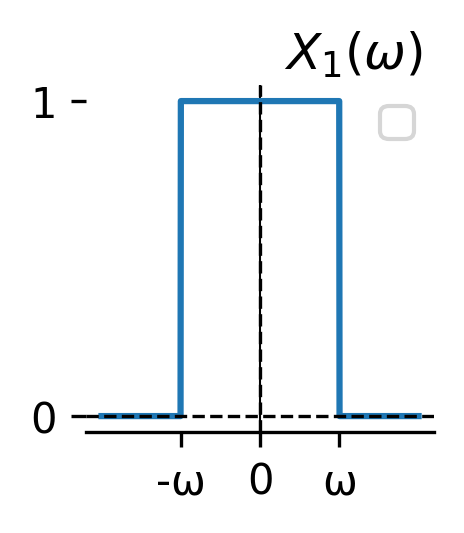
\includegraphics[width=0.4\columnwidth, height=2.5cm]{figs/plot.png}\hfill
    \begin{tabular}{c}
        {\sffamily\raisebox{1.75cm}{*}} 
    \end{tabular}\hfill
    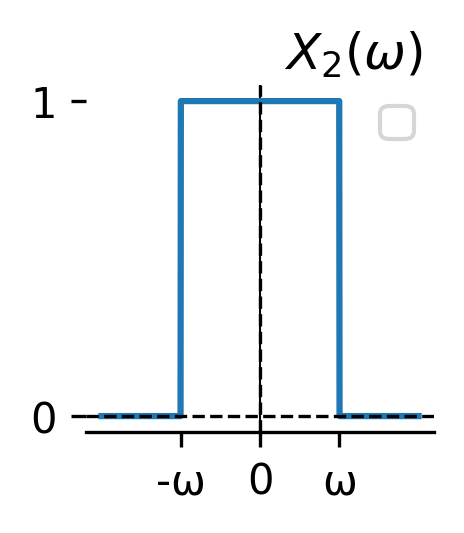
\includegraphics[width=0.4\columnwidth, height=2.5cm]{figs/plot4.png}
    
    \caption{}
    \label{fig:overall}
\end{figure}

\begin{align}
\left(\frac{\sin(\omega t)}{\pi t}\right)^2  \xleftrightarrow{\mathcal{F}} X_3(\omega) 
\end{align}
\begin{figure}[h!]
    \centering
    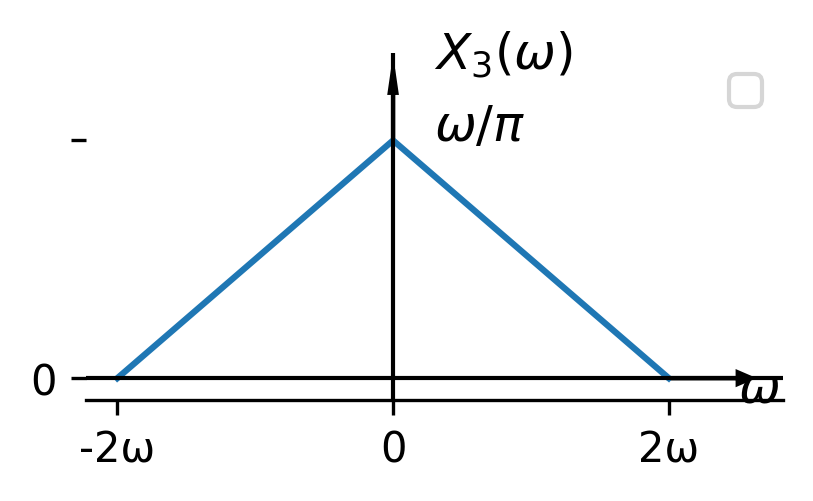
\includegraphics[width=0.5\columnwidth, height=3cm]{figs/plot1.png}
    \caption{}
    \label{fig:sr11}
\end{figure}
\begin{align}
\pi\left(\frac{\sin(\omega t)}{\pi t}\right)^2 \xleftrightarrow{\mathcal{F}} X_4(\omega)
\end{align}
\begin{figure}[h!]
    \centering
    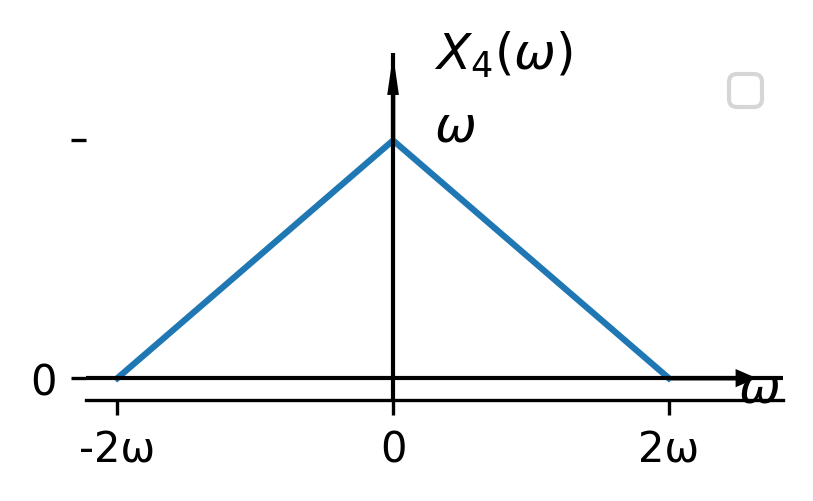
\includegraphics[width=0.5\columnwidth, height=3cm]{figs/plot2.png}
    \caption{}
    \label{fig:sr12}
\end{figure}
    \begin{align}
\text{From modulating property:} \nonumber \\
        f(t) \cos(\omega_0 t) \xleftrightarrow{\mathcal{F}} \frac{1}{2} \left[F(\omega + \omega_0) + F(\omega - \omega_0)\right]
    \end{align}

    \begin{align}
        H(\omega) &= \frac{1}{2} \left[F(\omega + 10\omega) + F(\omega - 10\omega)\right]
    \end{align}

\begin{figure}[h!]
    \centering
    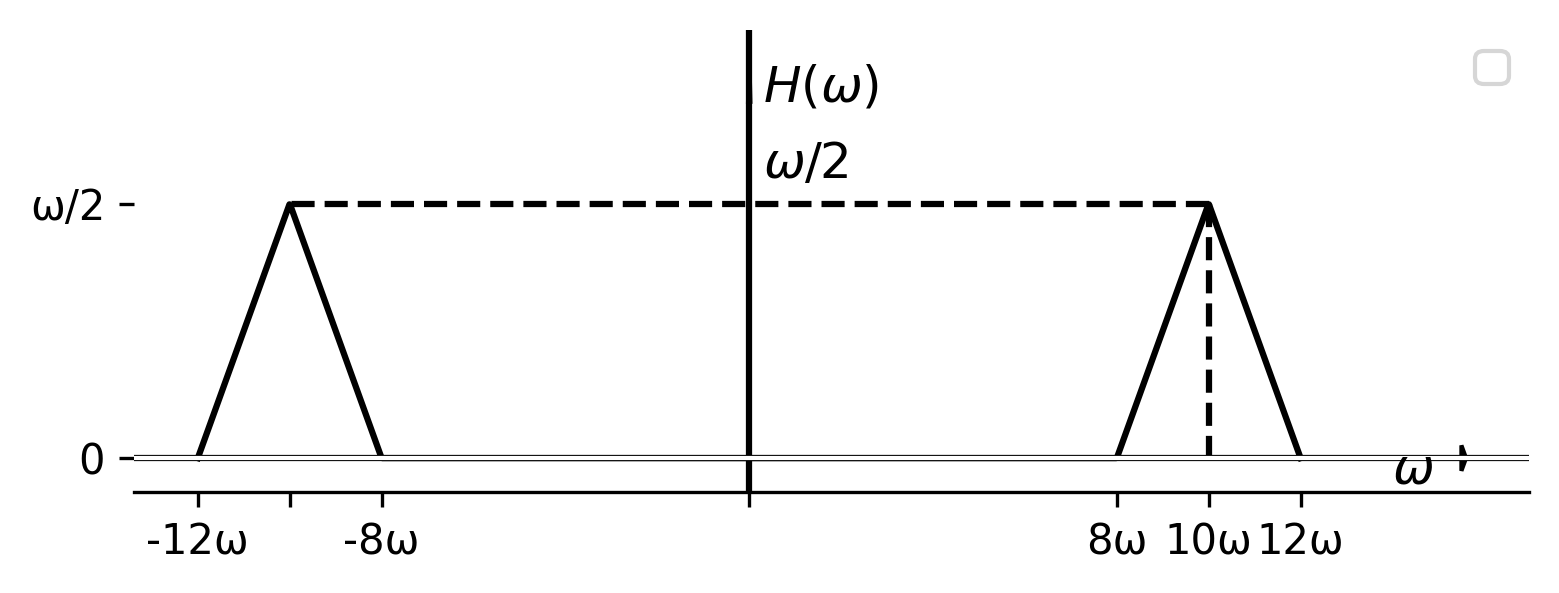
\includegraphics[width=0.7\columnwidth,height=2.5cm]{figs/plot3.png}
    \caption{}
    \label{fig:sr13}
\end{figure}
\begin{equation}
    \frac{\frac{\omega}{2} - 0}{10\omega - 12\omega} = \frac{|H(10.5\omega)| - 0}{10.5\omega - 12\omega}
\end{equation}

\begin{align}
A = |H(10.5\omega)| &= \frac{3}{8}\omega \quad \text{and} \quad  \theta= \angle H(10.5\omega) = 0^\circ
\end{align}

The output \(y(t)\):
\begin{align}
y(t) &= \frac{3}{8}\omega \cdot 10 \cos(10.5 \omega t) \\
&= \frac{15}{4}\omega \cos(10.5 \omega t)
\end{align}
\begin{figure}[h!]
    \centering
    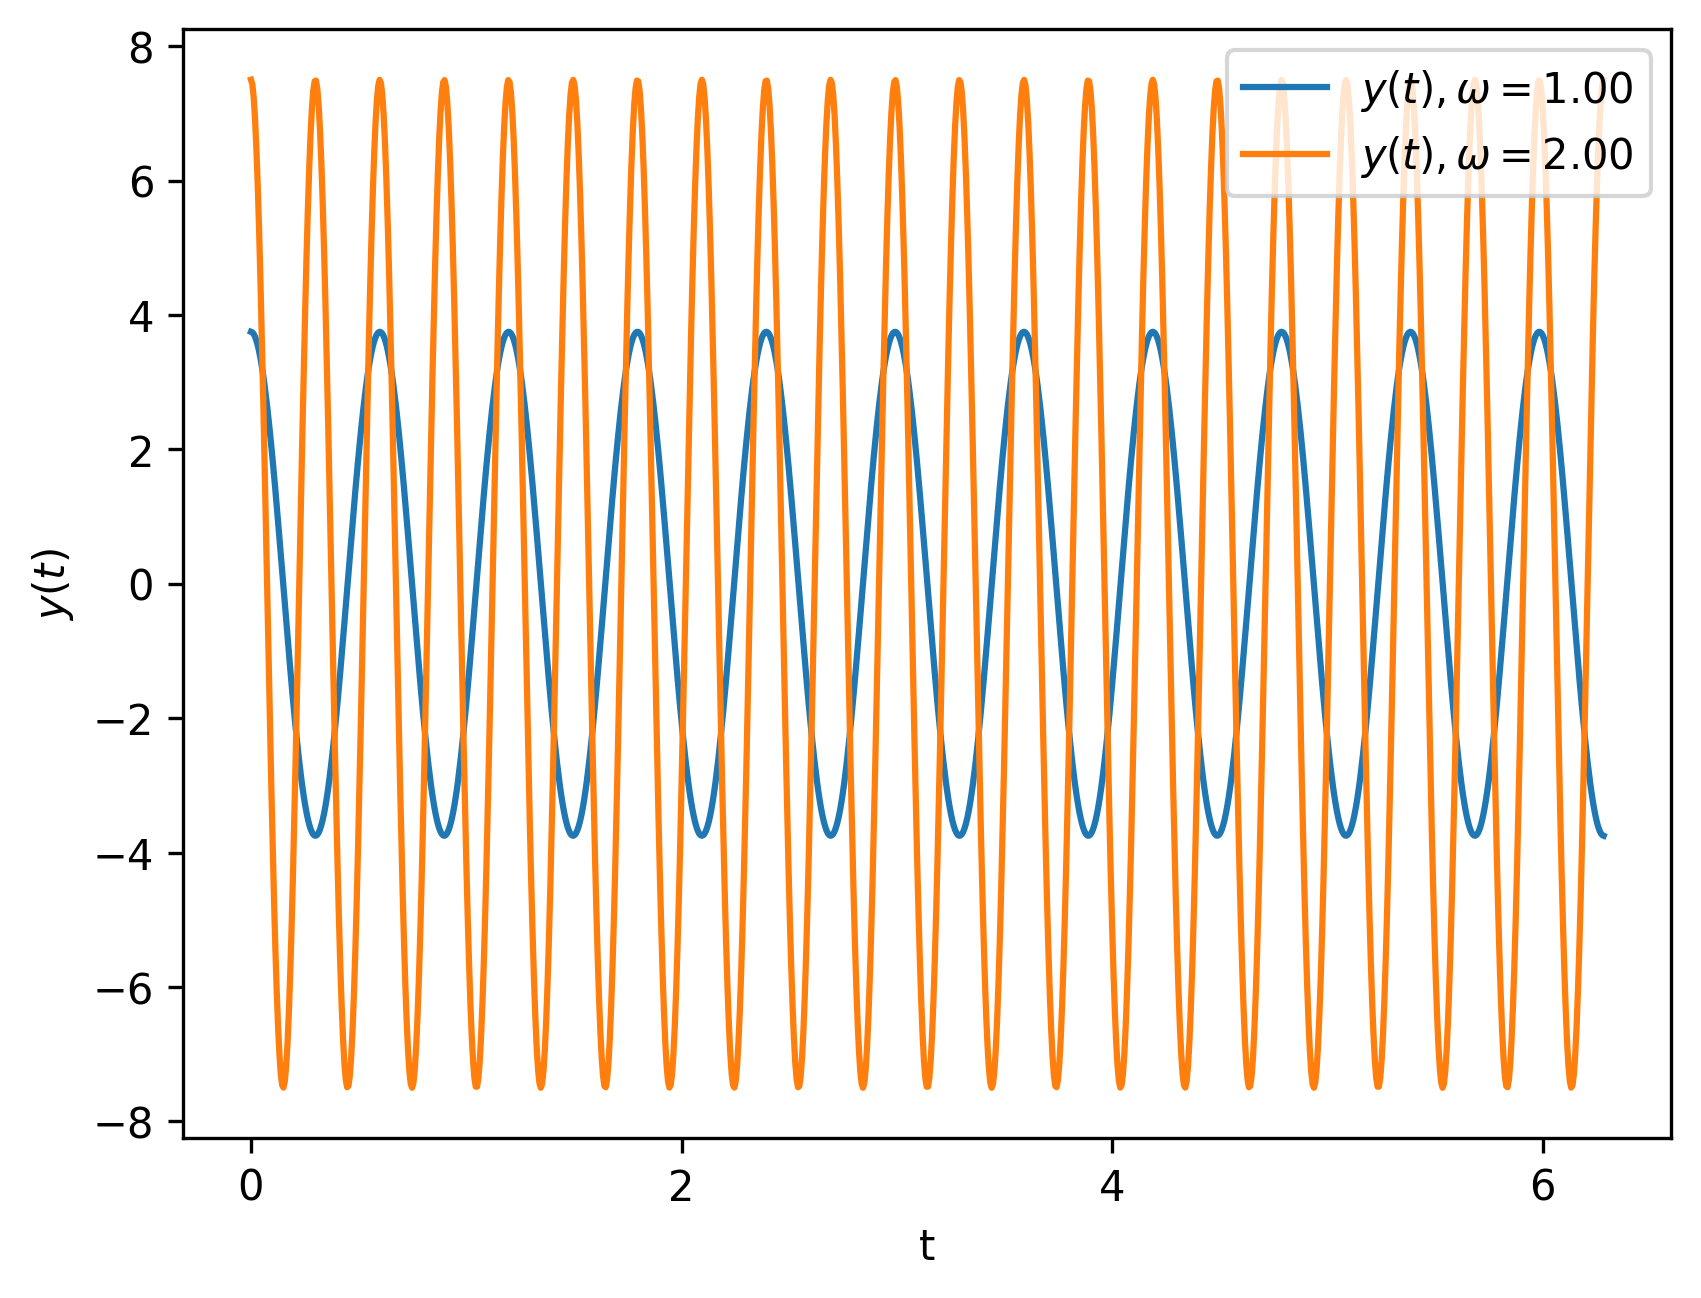
\includegraphics[width=\columnwidth]{figs/plot5.png}
    \caption{}
    \label{fig:sr14}
\end{figure}
\end{document}


\newpage

\item The continuous time signal $x(t)$ is described by:
\begin{align}
x(t)=
    \begin{cases}
        1, & \text{if } 0\: {\displaystyle \leq }\:t\:{\displaystyle \leq }\:1\\
        0, & \text{elsewhere}
    \end{cases} 
\end{align}
If $y(t)$ represents $x(t)$ convolved with itself, which of the following options is/are TRUE?
\begin{enumerate}[label = \Alph*]
    \item $y(t)$ = 0 for all $t<0$\\
    \item $y(t)$ = 0 for all $t>1$\\
    \item $y(t)$ = 0 for all $t>3$\\
    \item $\int_{0.1}^{0.75} \frac{dy(t)}{dt}\: \text{dt} \neq 0$
\end{enumerate}
\solution
\newpage

\item The Z-transform of a discrete signal $x\brak{n}$ is
\begin{align}
X\brak{z}=\dfrac{4z}{\brak{z-\dfrac{1}{5}} \brak{z-\dfrac{2}{3}} \brak{z-3}} \text{ with ROC= }R
\end{align}
Which one of the following statements is TRUE?
\begin{enumerate}[label = (\alph*)]
     \item Discrete time Fourier transform of $x\sbrak{n}$ converges if $R$ is $|z|>3$\\
     \item Discrete time Fourier transform of $x\sbrak{n}$ converges if $ R$ is $\dfrac{2}{3}<|z|<3$\\
     \item Discrete time Fourier transform of $x\sbrak{n}$ converges if $R$ is such that $x\sbrak{n}$ is a left-sided sequence.\\
     \item Discrete time Fourier transform of $x\sbrak{n}$ converges if $R$ is such that $x\sbrak{n}$is a right-sided sequence.\\
 \end{enumerate} \hfill{GATE EE 2023}	\\
 \solution
 \input{2023/EE/19/1.tex}
 \newpage
 
\item The phase margin of the transfer function $G(s) = \frac{2(1-s)}{(1+s)^2}$ is \rule{1cm}{0.15mm} degrees. (rounded off to the nearest integer). \hfill (GATE IN 2023)\\
\solution
\input{2023/IN/50/in_50.tex}
\newpage
\item Consider the second-order linear differential equation
\[x^2\frac{d^2y}{dx^2}+x\frac{dy}{dx}-y=0, \; x\geq 1\]
with the initial conditions \[y(x=1)=6,\; \;\; \frac{dy}{dx}\big{|}_{x=1}=2.\]
Then the value of $y$ at $x=2$ is \rule{2cm}{0.1mm}.\\{\hfill{GATE ME 2023}}\\
\solution
\iffalse
\let\negmedspace\undefined
\let\negthickspace\undefined
\documentclass[journal,12pt,twocolumn]{IEEEtran}
\usepackage{cite}
\usepackage{amsmath,amssymb,amsfonts}
\usepackage{graphicx}
\usepackage{textcomp}
\usepackage{xcolor}
\usepackage{txfonts}
\usepackage{listings}
\usepackage{enumitem}
\usepackage{mathtools}
\usepackage{gensymb}
\usepackage{comment}
\usepackage[breaklinks=true]{hyperref}
\usepackage{tkz-euclide} 
\usepackage{listings}
\usepackage{gvv}                                        
\def\inputGnumericTable{}                                 
\usepackage[latin1]{inputenc}                                
\usepackage{color}                                            
\usepackage{array}                                            
\usepackage{longtable}                                       
\usepackage{calc}                                             
\usepackage{multirow}                                         
\usepackage{hhline}                                           
\usepackage{ifthen}                                           
\usepackage{lscape}
\usepackage[export]{adjustbox}

\newtheorem{theorem}{Theorem}[section]
\newtheorem{problem}{Problem}
\newtheorem{proposition}{Proposition}[section]
\newtheorem{lemma}{Lemma}[section]
\newtheorem{corollary}[theorem]{Corollary}
\newtheorem{example}{Example}[section]
\newtheorem{definition}[problem]{Definition}
\newcommand{\BEQA}{\begin{eqnarray}}
\newcommand{\EEQA}{\end{eqnarray}}
\newcommand{\define}{\stackrel{\triangle}{=}}
\newtheorem{rem}{Remark}

\begin{document}
\parindent 0px
\bibliographystyle{IEEEtran}

\vspace{3cm}

\title{}
\author{EE23BTECH11042 -  Khusinadha Naik$^{*}$
}
\maketitle
\newpage
\bigskip

% \renewcommand{\thefigure}{\theenumi}
% \renewcommand{\thetable}{\theenumi}


\noindent \textbf{26.} \hspace{2pt}A causal, discrete time system is described by the difference equation $y[n] = 0.5 y[n-1] + x[n]$, for all $n$, where $y[n]$ denotes the output sequence and $x[n]$ denotes the input sequence. Which of the following statements is/are TRUE?
\begin{flushright}
\hfill(GATE 2023 BM)
\end{flushright}
\begin{enumerate}[label = (\alph*)]
	\item The system has an impulse response described by $0.5^{n} u[-n]$ where $u[n]$ is the  
unit step sequence. 	\label{option:GATE.2023.BM.26.1}	
	\item The system is stable in the bounded input, bounded output sense.		\label{option:GATE.2023.BM.26.2}
	\item The system has an infinite number of non-zero samples in its impulse response	\label{option:GATE.2023.BM.26.3}
	\item The system has a finite number of non-zero samples in its impulse response.	\label{option:GATE.2023.BM.26.4}
\end{enumerate}

\noindent \textbf{Ans.}\\
\fi
\begin{table}[h]
\centering
\begin{tabular}{|c|c|c|}
        \hline
        \textbf{Parameter} & \textbf{Value} & \textbf{Description} \\
        \hline
        $x[n]$ & ? & Input Sequence \\
        \hline
        $y[n]$ & ? & Output Sequence \\
        \hline
\end{tabular}
\caption{Input parameters table}
\label{tab:GATE.2023.BM.26.1}





\end{table}
\begin{align}
y[n] = 0.5y[n-1] + x[n] 
\end{align}

Taking $Z$-Transform 
\begin{align}
Y\brak{z} &= 0.5z^{-1}Y\brak{z} + X\brak{z} \\
\implies \frac{Y\brak{z}}{X\brak{z}} &= \frac{1}{1 - 0.5z^{-1}} = H\brak{z} 
\end{align}
If $x[n]$ is impulse input 
\begin{align}
\implies &Y\brak{z} = H\brak{z} = \frac{1}{1 - 0.5z^{-1}}  \label{eq:GATE.2023.BM.26.4}
\end{align}
From \eqref{eq:GATE.2023.BM.26.4} pole lies at $z = 0.5$
\begin{align}
a^{n}u\brak{n} \xleftrightarrow{\mathcal{Z}} &\frac{1}{1 - az^{-1}} \quad , \abs{z} > a \label{eq:GATE.2023.BM.26.5}
\end{align}

From \eqref{eq:GATE.2023.BM.26.4} , \eqref{eq:GATE.2023.BM.26.5}
\begin{align}
h[n] = 0.5^{n}u[n] \quad , \abs{z} > 0.5 \label{eq:GATE.2023.BM.26.6}
\end{align}


\pagebreak
Plotting $h[n]$ vs $n$
\begin{figure}[h]
    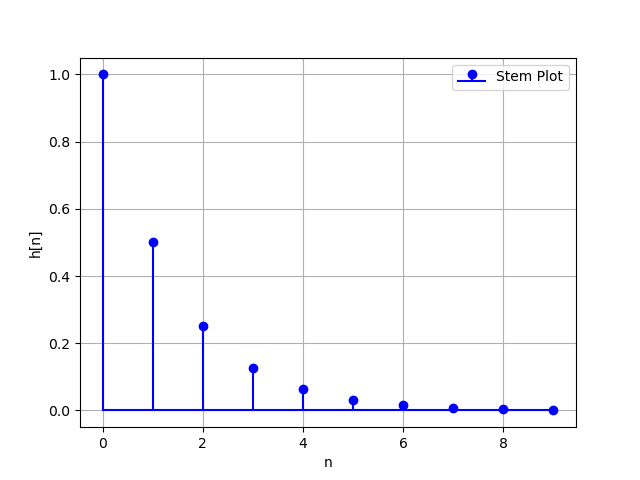
\includegraphics[width=0.5\textwidth]{2023/BM/26/figs/fig1.png}
    \caption{Plot of $h[n]$ vs $n$}
    \label{fig:GATE.2023.BM.26.1}
\end{figure}

\begin{enumerate}
\item From \eqref{eq:GATE.2023.BM.26.6} , \ref{option:GATE.2023.BM.26.1} is wrong
\item As pole lies within unit circle \ref{option:GATE.2023.BM.26.2} is true
\item From \eqref{eq:GATE.2023.BM.26.6} and \figref{fig:GATE.2023.BM.26.1} ,\ref{option:GATE.2023.BM.26.3} is true and hence
\item \ref{option:GATE.2023.BM.26.4} is false 
\end{enumerate}





%\end{document}

\newpage
\item The transfer function of a measuring instrument is \\
$$G_m(s) = \frac{1.05}{2s+1}exp(-s)$$
At time $t = 0$, a step change of +1 unit is introduced in the input of this instrument.The time taken by the instrument to show an increase of 1 unit in its output is(rounded off to two decimal places).\\ \hfill (GATE CH 2023)
\solution
\iffalse
\let\negmedspace\undefined
\let\negthickspace\undefined
\documentclass[journal,12pt,twocolumn]{IEEEtran}
\usepackage{cite}
\usepackage{amsmath,amssymb,amsfonts,amsthm}
\usepackage{algorithmic}
\usepackage{graphicx}
\usepackage{textcomp}
\usepackage{xcolor}
\usepackage{txfonts}
\usepackage{listings}
\usepackage{enumitem}
\usepackage{mathtools}
\usepackage{gensymb}
\usepackage{comment}
\usepackage[breaklinks=true]{hyperref}
\usepackage{tkz-euclide} 
\usepackage{listings}
\usepackage{gvv}                                        
\def\inputGnumericTable{}                                 
\usepackage[latin1]{inputenc}                                
\usepackage{color}                                            
\usepackage{array}                                            
\usepackage{longtable}                                       
\usepackage{calc}                                             
\usepackage{multirow}                                         
\usepackage{hhline}                                           
\usepackage{ifthen}                                           
\usepackage{lscape}
\usepackage{amsmath}
\usepackage{caption}

\newtheorem{theorem}{Theorem}[section]
\newtheorem{problem}{Problem}
\newtheorem{proposition}{Proposition}[section]
\newtheorem{lemma}{Lemma}[section]
\newtheorem{corollary}[theorem]{Corollary}
\newtheorem{example}{Example}[section]
\newtheorem{definition}[problem]{Definition}
\newcommand{\BEQA}{\begin{eqnarray}}
\newcommand{\EEQA}{\end{eqnarray}}
\newcommand{\define}{\stackrel{\triangle}{=}}
\theoremstyle{remark}
\newtheorem{rem}{Remark}
\begin{document}

\bibliographystyle{IEEEtran}
\vspace{3cm}

\title{GATE: CH-62 2023}
\author{EE23BTECH11038 - Rohith Madhani$^{*}$% <-this % stops a space
}
\maketitle
\newpage
\bigskip
\renewcommand{\thefigure}{\theenumi}
\renewcommand{\thetable}{\theenumi}

\textbf{Question :} The transfer function of a measuring instrument is \\
$$G_m(s) = \frac{1.05}{2s+1}exp(-s)$$
At time $t = 0$, a step change of +1 unit is introduced in the input of this instrument.The time taken by the instrument to show an increase of 1 unit in its output is(rounded off to two decimal places). \\ \hfill(GATE CH 2023) \\
\solution
\fi

\begin{table}[!h] 
\centering
%%%%%%%%%%%%%%%%%%%%%%%%%%%%%%%%%%%%%%%%%%%%%%%%%%%%%%%%%%%%%%%%%%%%%%
%%                                                                  %%
%%  This is the header of a LaTeX2e file exported from Gnumeric.    %%
%%                                                                  %%
%%  This file can be compiled as it stands or included in another   %%
%%  LaTeX document. The table is based on the longtable package so  %%
%%  the longtable options (headers, footers...) can be set in the   %%
%%  preamble section below (see PRAMBLE).                           %%
%%                                                                  %%
%%  To include the file in another, the following two lines must be %%
%%  in the including file:                                          %%
%%        \def\inputGnumericTable{}                                 %%
%%  at the beginning of the file and:                               %%
%%        \input{name-of-this-file.tex}                             %%
%%  where the table is to be placed. Note also that the including   %%
%%  file must use the following packages for the table to be        %%
%%  rendered correctly:                                             %%
%%    \usepackage[latin1]{inputenc}                                 %%
%%    \usepackage{color}                                            %%
%%    \usepackage{array}                                            %%
%%    \usepackage{longtable}                                        %%
%%    \usepackage{calc}                                             %%
%%    \usepackage{multirow}                                         %%
%%    \usepackage{hhline}                                           %%
%%    \usepackage{ifthen}                                           %%
%%  optionally (for landscape tables embedded in another document): %%
%%    \usepackage{lscape}                                           %%
%%                                                                  %%
%%%%%%%%%%%%%%%%%%%%%%%%%%%%%%%%%%%%%%%%%%%%%%%%%%%%%%%%%%%%%%%%%%%%%%



%%  This section checks if we are begin input into another file or  %%
%%  the file will be compiled alone. First use a macro taken from   %%
%%  the TeXbook ex 7.7 (suggestion of Han-Wen Nienhuys).            %%
\def\ifundefined#1{\expandafter\ifx\csname#1\endcsname\relax}


%%  Check for the \def token for inputed files. If it is not        %%
%%  defined, the file will be processed as a standalone and the     %%
%%  preamble will be used.                                          %%
\ifundefined{inputGnumericTable}

%%  We must be able to close or not the document at the end.        %%
	\def\gnumericTableEnd{\end{document}}


%%%%%%%%%%%%%%%%%%%%%%%%%%%%%%%%%%%%%%%%%%%%%%%%%%%%%%%%%%%%%%%%%%%%%%
%%                                                                  %%
%%  This is the PREAMBLE. Change these values to get the right      %%
%%  paper size and other niceties.                                  %%
%%                                                                  %%
%%%%%%%%%%%%%%%%%%%%%%%%%%%%%%%%%%%%%%%%%%%%%%%%%%%%%%%%%%%%%%%%%%%%%%

	\documentclass[12pt%
			  %,landscape%
                    ]{report}
       \usepackage[latin1]{inputenc}
       \usepackage{fullpage}
       \usepackage{color}
       \usepackage{array}
       \usepackage{longtable}
       \usepackage{calc}
       \usepackage{multirow}
       \usepackage{hhline}
       \usepackage{ifthen}

	\begin{document}


%%  End of the preamble for the standalone. The next section is for %%
%%  documents which are included into other LaTeX2e files.          %%
\else

%%  We are not a stand alone document. For a regular table, we will %%
%%  have no preamble and only define the closing to mean nothing.   %%
    \def\gnumericTableEnd{}

%%  If we want landscape mode in an embedded document, comment out  %%
%%  the line above and uncomment the two below. The table will      %%
%%  begin on a new page and run in landscape mode.                  %%
%       \def\gnumericTableEnd{\end{landscape}}
%       \begin{landscape}


%%  End of the else clause for this file being \input.              %%
\fi

%%%%%%%%%%%%%%%%%%%%%%%%%%%%%%%%%%%%%%%%%%%%%%%%%%%%%%%%%%%%%%%%%%%%%%
%%                                                                  %%
%%  The rest is the gnumeric table, except for the closing          %%
%%  statement. Changes below will alter the table's appearance.     %%
%%                                                                  %%
%%%%%%%%%%%%%%%%%%%%%%%%%%%%%%%%%%%%%%%%%%%%%%%%%%%%%%%%%%%%%%%%%%%%%%

\providecommand{\gnumericmathit}[1]{#1} 
%%  Uncomment the next line if you would like your numbers to be in %%
%%  italics if they are italizised in the gnumeric table.           %%
%\renewcommand{\gnumericmathit}[1]{\mathit{#1}}
\providecommand{\gnumericPB}[1]%
{\let\gnumericTemp=\\#1\let\\=\gnumericTemp\hspace{0pt}}
 \ifundefined{gnumericTableWidthDefined}
        \newlength{\gnumericTableWidth}
        \newlength{\gnumericTableWidthComplete}
        \newlength{\gnumericMultiRowLength}
        \global\def\gnumericTableWidthDefined{}
 \fi
%% The following setting protects this code from babel shorthands.  %%
 \ifthenelse{\isundefined{\languageshorthands}}{}{\languageshorthands{english}}
%%  The default table format retains the relative column widths of  %%
%%  gnumeric. They can easily be changed to c, r or l. In that case %%
%%  you may want to comment out the next line and uncomment the one %%
%%  thereafter                                                      %%
\providecommand\gnumbox{\makebox[0pt]}
%%\providecommand\gnumbox[1][]{\makebox}

%% to adjust positions in multirow situations                       %%
\setlength{\bigstrutjot}{\jot}
\setlength{\extrarowheight}{\doublerulesep}

%%  The \setlongtables command keeps column widths the same across  %%
%%  pages. Simply comment out next line for varying column widths.  %%
\setlongtables

\setlength\gnumericTableWidth{%
	44pt+%
	200pt+%
	60pt+%
0pt}
\def\gumericNumCols{3}
\setlength\gnumericTableWidthComplete{\gnumericTableWidth+%
         \tabcolsep*\gumericNumCols*2+\arrayrulewidth*\gumericNumCols}
\ifthenelse{\lengthtest{\gnumericTableWidthComplete > \linewidth}}%
         {\def\gnumericScale{1*\ratio{\linewidth-%
                        \tabcolsep*\gumericNumCols*2-%
                        \arrayrulewidth*\gumericNumCols}%
{\gnumericTableWidth}}}%
{\def\gnumericScale{1}}

%%%%%%%%%%%%%%%%%%%%%%%%%%%%%%%%%%%%%%%%%%%%%%%%%%%%%%%%%%%%%%%%%%%%%%
%%                                                                  %%
%% The following are the widths of the various columns. We are      %%
%% defining them here because then they are easier to change.       %%
%% Depending on the cell formats we may use them more than once.    %%
%%                                                                  %%
%%%%%%%%%%%%%%%%%%%%%%%%%%%%%%%%%%%%%%%%%%%%%%%%%%%%%%%%%%%%%%%%%%%%%%

\ifthenelse{\isundefined{\gnumericColA}}{\newlength{\gnumericColA}}{}\settowidth{\gnumericColA}{\begin{tabular}{@{}p{44pt*\gnumericScale}@{}}x\end{tabular}}
\ifthenelse{\isundefined{\gnumericColB}}{\newlength{\gnumericColB}}{}\settowidth{\gnumericColB}{\begin{tabular}{@{}p{200pt*\gnumericScale}@{}}x\end{tabular}}
\ifthenelse{\isundefined{\gnumericColC}}{\newlength{\gnumericColC}}{}\settowidth{\gnumericColC}{\begin{tabular}{@{}p{60pt*\gnumericScale}@{}}x\end{tabular}}

\begin{tabular}[c]{%
	b{\gnumericColA}%
	b{\gnumericColB}%
	b{\gnumericColC}%
	}

%%%%%%%%%%%%%%%%%%%%%%%%%%%%%%%%%%%%%%%%%%%%%%%%%%%%%%%%%%%%%%%%%%%%%%
%%  The longtable options. (Caption, headers... see Goosens, p.124) %%
%	\caption{The Table Caption.}             \\	%
% \hline	% Across the top of the table.
%%  The rest of these options are table rows which are placed on    %%
%%  the first, last or every page. Use \multicolumn if you want.    %%

%%  Header for the first page.                                      %%
%	\multicolumn{3}{c}{The First Header} \\ \hline 
%	\multicolumn{1}{c}{colTag}	%Column 1
%	&\multicolumn{1}{c}{colTag}	%Column 2
%	&\multicolumn{1}{c}{colTag}	\\ \hline %Last column
%	\endfirsthead

%%  The running header definition.                                  %%
%	\hline
%	\multicolumn{3}{l}{\ldots\small\slshape continued} \\ \hline
%	\multicolumn{1}{c}{colTag}	%Column 1
%	&\multicolumn{1}{c}{colTag}	%Column 2
%	&\multicolumn{1}{c}{colTag}	\\ \hline %Last column
%	\endhead

%%  The running footer definition.                                  %%
%	\hline
%	\multicolumn{3}{r}{\small\slshape continued\ldots} \\
%	\endfoot

%%  The ending footer definition.                                   %%
%	\multicolumn{3}{c}{That's all folks} \\ \hline 
%	\endlastfoot
%%%%%%%%%%%%%%%%%%%%%%%%%%%%%%%%%%%%%%%%%%%%%%%%%%%%%%%%%%%%%%%%%%%%%%

\hhline{|-|-|-|}
	 \multicolumn{1}{|p{\gnumericColA}|}%
	{\gnumericPB{\centering}\gnumbox{Parameter}}
	&\multicolumn{1}{p{\gnumericColB}|}%
	{\gnumericPB{\centering}\gnumbox{Description}}
	&\multicolumn{1}{p{\gnumericColC}|}%
	{\gnumericPB{\centering}\gnumbox{Value}}
\\
\hhline{|-|-|-|}
	 \multicolumn{1}{|p{\gnumericColA}|}%
	{\gnumericPB{\centering}\gnumbox{$G_m(s)$}}
	&\multicolumn{1}{p{\gnumericColB}|}%
	{\gnumericPB{\centering}\gnumbox{Transfer function}}
	&\multicolumn{1}{p{\gnumericColC}|}%
	{\gnumericPB{\centering}\gnumbox{$\frac{Y(s)}{U(s)}$}}
\\
\hhline{|-|-|-|}
	 \multicolumn{1}{|p{\gnumericColA}|}%
	{\gnumericPB{\centering}\gnumbox{Y(s)}}
	&\multicolumn{1}{p{\gnumericColB}|}%
	{\gnumericPB{\centering}\gnumbox{Laplace transform of the output}}
	&\multicolumn{1}{p{\gnumericColC}|}%
	{\gnumericPB{\centering}\gnumbox{?}}
\\
\hhline{|-|-|-|}
	 \multicolumn{1}{|p{\gnumericColA}|}%
	{\gnumericPB{\centering}\gnumbox{U(s)}}
	&\multicolumn{1}{p{\gnumericColB}|}%
	{\gnumericPB{\centering}\gnumbox{Laplace transform of the input}}
	&\multicolumn{1}{p{\gnumericColC}|}%
	{\gnumericPB{\centering}\gnumbox{$\frac{1}{s}$}}
\\
\hhline{|-|-|-|}
\end{tabular}

\ifthenelse{\isundefined{\languageshorthands}}{}{\languageshorthands{\languagename}}
\gnumericTableEnd
\caption{Given parameters}
\label{table:gate23ch62}
\end{table}

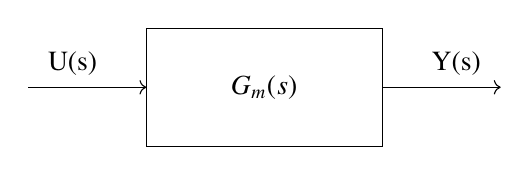
\begin{tikzpicture}
\centering
    % Draw the main box
    \node[draw, minimum width=3cm, minimum height=1.5cm] (box) at (0,0) {$G_m(s)$};
    
    % Draw the input arrow
    \draw[->] (-3,0) -- (-1.5,0);
    
    % Draw the output arrow
    \draw[->] (1.5,0) -- (3,0);
    
    % Label the input arrow
    \node[anchor=east] at (-2,0.3) {U(s)};
    
    % Label the output arrow
    \node[anchor=west] at (2,0.3) {Y(s)};
\end{tikzpicture}

\begin{align}
    G_m(s) &= \frac{1.05}{2s+1}e^{-s} \\
    \because Y(s) &= G_m(s).U(s) \\
    \implies Y(s) &= \frac{1}{s}.\frac{1.05}{2s+1}e^{-s}
\end{align}

By splitting into partial fractions,we get
\begin{align}
    Y(s) &= \sbrak{\frac{1.05}{s} - \frac{1.05}{s+0.5}}e^{-s}
\end{align}

As we know,
\begin{align}
    \mathcal{L}[e^{-at}] &\system{} \frac{1}{s+a} \\
    \mathcal{L}[f(t-1)] &\system{} e^{-s}F(s)
\end{align}

By taking inverse laplce we get,

\begin{align}
    y(t) &= 1.05\sbrak{1-e^{\frac{-(t-1)}{2}}}u(t-1) \\
    \frac{1}{1.05} &= 1-e^{\frac{-(t-1)}{2}} \\
    \frac{-(t-1)}{2} &= \ln(\frac{0.05}{1.05}) \\
    \implies t &= 7.073 
\end{align}

\begin{figure}[h]
    \centering
    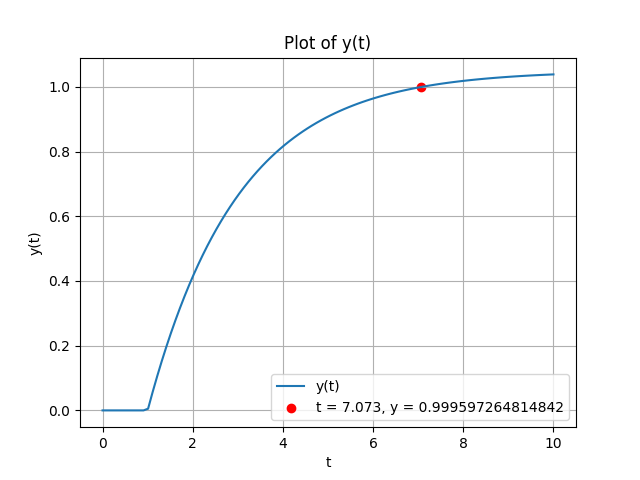
\includegraphics[width=\columnwidth]{2023/CH/62/figs/fig1.png}
    \caption{y(t) = $1.05\sbrak{1-e^{\frac{t-1}{2}}}$}
    \label{fig:gate23ch62}
\end{figure}

%\end{document}

\newpage
\item
The laplace transform of $x_1(t)$ = $e^{-t}u(t)$ is $X_1(s)$, where $u(t)$ is the unit step function. The laplace transform of $x_2(t) = e^tu(-t)$ is $X_2(s)$. Which one of the following statements is TRUE?
\begin{enumerate}
    \item The region of convergence of $X_1(s)$ is $Re(s) \geq 0$
    \item The region of convergence of $X_2(s)$ is confined to the left half-plane of s.
    \item The region of convergence of $X_1(s)$ is confined to the right half-plane of s.
    \item the imaginary axis in the s-plane is included in both the region of convergence of $X_1(s)$ and the region of convergence of $X_2(s)$.
\end{enumerate} \hfill(GATE BM 2023)\\
\solution
\input{2023/BM/39/bm39.tex}
\newpage
\item Given that $\frac{dy}{dx}=2x+y$ and $y=1$,when $x=0$ Using Runge-Kutta fourth order method,the value of $y$ at $x=0.2$ is \hfill(GATE 2023 AG 50) \\
\solution

\item The magnitude and phase plots shown in the figure match with the transfer-
function
\begin{figure}[h]
    \centering
    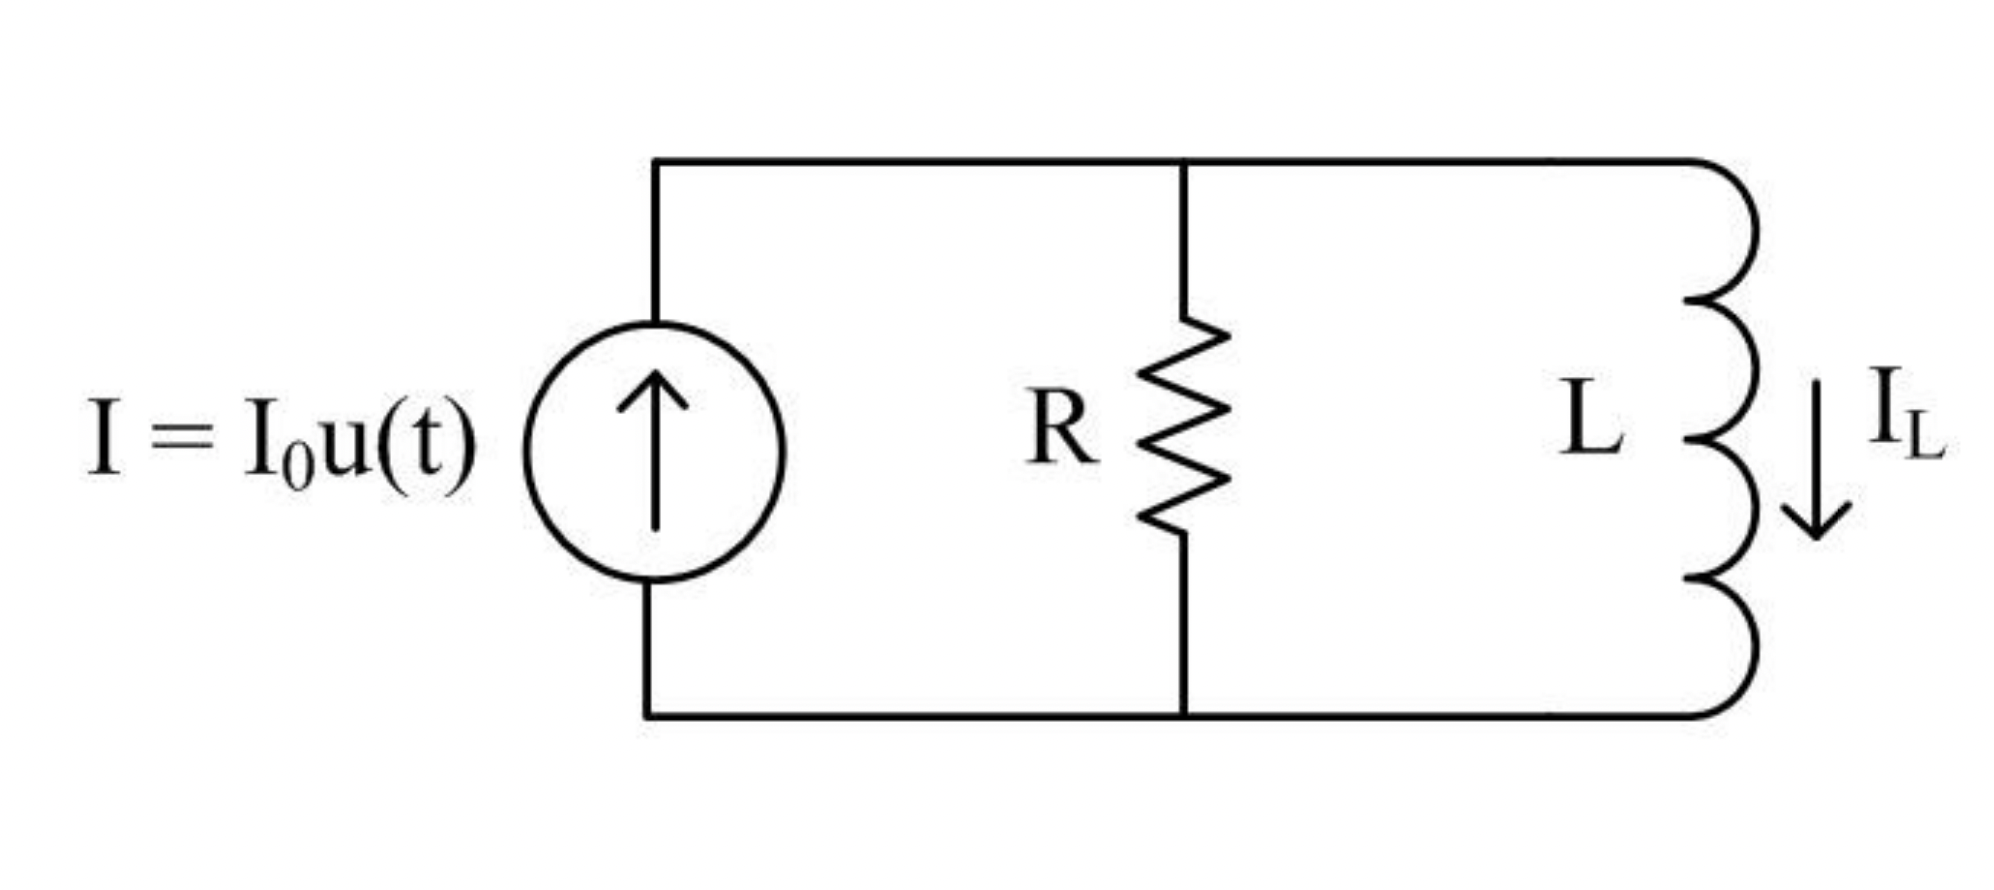
\includegraphics[width=\columnwidth]{2023/IN/43/figs/question.png}
\end{figure}\\
\begin{enumerate}
\item $\frac{10000}{s^2+2s+10000}$\\
\item $\frac{10000}{s^2+2s+10000}e^{-0.05s}$\\
\item $\frac{10000}{s^2+2s+10000}e^{-0.5\times10^{-12}s}$\\
\item $\frac{100}{s^2+2s+100}$
\end{enumerate}
\hfill{(GATE IN 2023)}
\solution
\iffalse
\let\negmedspace\undefined
\let\negthickspace\undefined
\documentclass[journal,12pt,onecolumn]{IEEEtran}
\usepackage{cite}
\usepackage{amsmath,amssymb,amsfonts,amsthm}
\usepackage{algorithmic}
\usepackage{graphicx}
\usepackage{textcomp}
\usepackage{xcolor}
\usepackage{txfonts}
\usepackage{listings}
\usepackage{enumitem}
\usepackage{mathtools}
\usepackage{gensymb}
\usepackage{comment}
\usepackage{caption}
\usepackage[breaklinks=true]{hyperref}
\usepackage{tkz-euclide} 
\usepackage{listings}
\usepackage{gvv}                                        
\def\inputGnumericTable{}                                 
\usepackage[latin1]{inputenc}                                
\usepackage{color}                                            
\usepackage{array}                                            
\usepackage{longtable}                                       
\usepackage{calc}                                             
\usepackage{multirow}                                         
\usepackage{hhline}                                           
\usepackage{ifthen}                                           
\usepackage{lscape}

\newtheorem{theorem}{Theorem}[section]
\newtheorem{problem}{Problem}
\newtheorem{proposition}{Proposition}[section]
\newtheorem{lemma}{Lemma}[section]
\newtheorem{corollary}[theorem]{Corollary}
\newtheorem{example}{Example}[section]
\newtheorem{definition}[problem]{Definition}
\newcommand{\BEQA}{\begin{eqnarray}}
\newcommand{\EEQA}{\end{eqnarray}}
\newcommand{\define}{\stackrel{\triangle}{=}}
\theoremstyle{remark}
\newtheorem{rem}{Remark}
\begin{document}

\bibliographystyle{IEEEtran}
\vspace{3cm}

\title{GATE IN 43}
\author{EE23BTECH11022 - G DILIP REDDY}
\maketitle

\bigskip

\renewcommand{\thefigure}{\arabic{figure}}
\renewcommand{\thetable}{\arabic{table}}
\textbf{Question}:\\
The magnitude and phase plots shown in the figure match with the transfer-
function
\begin{figure}[h]
    \centering
    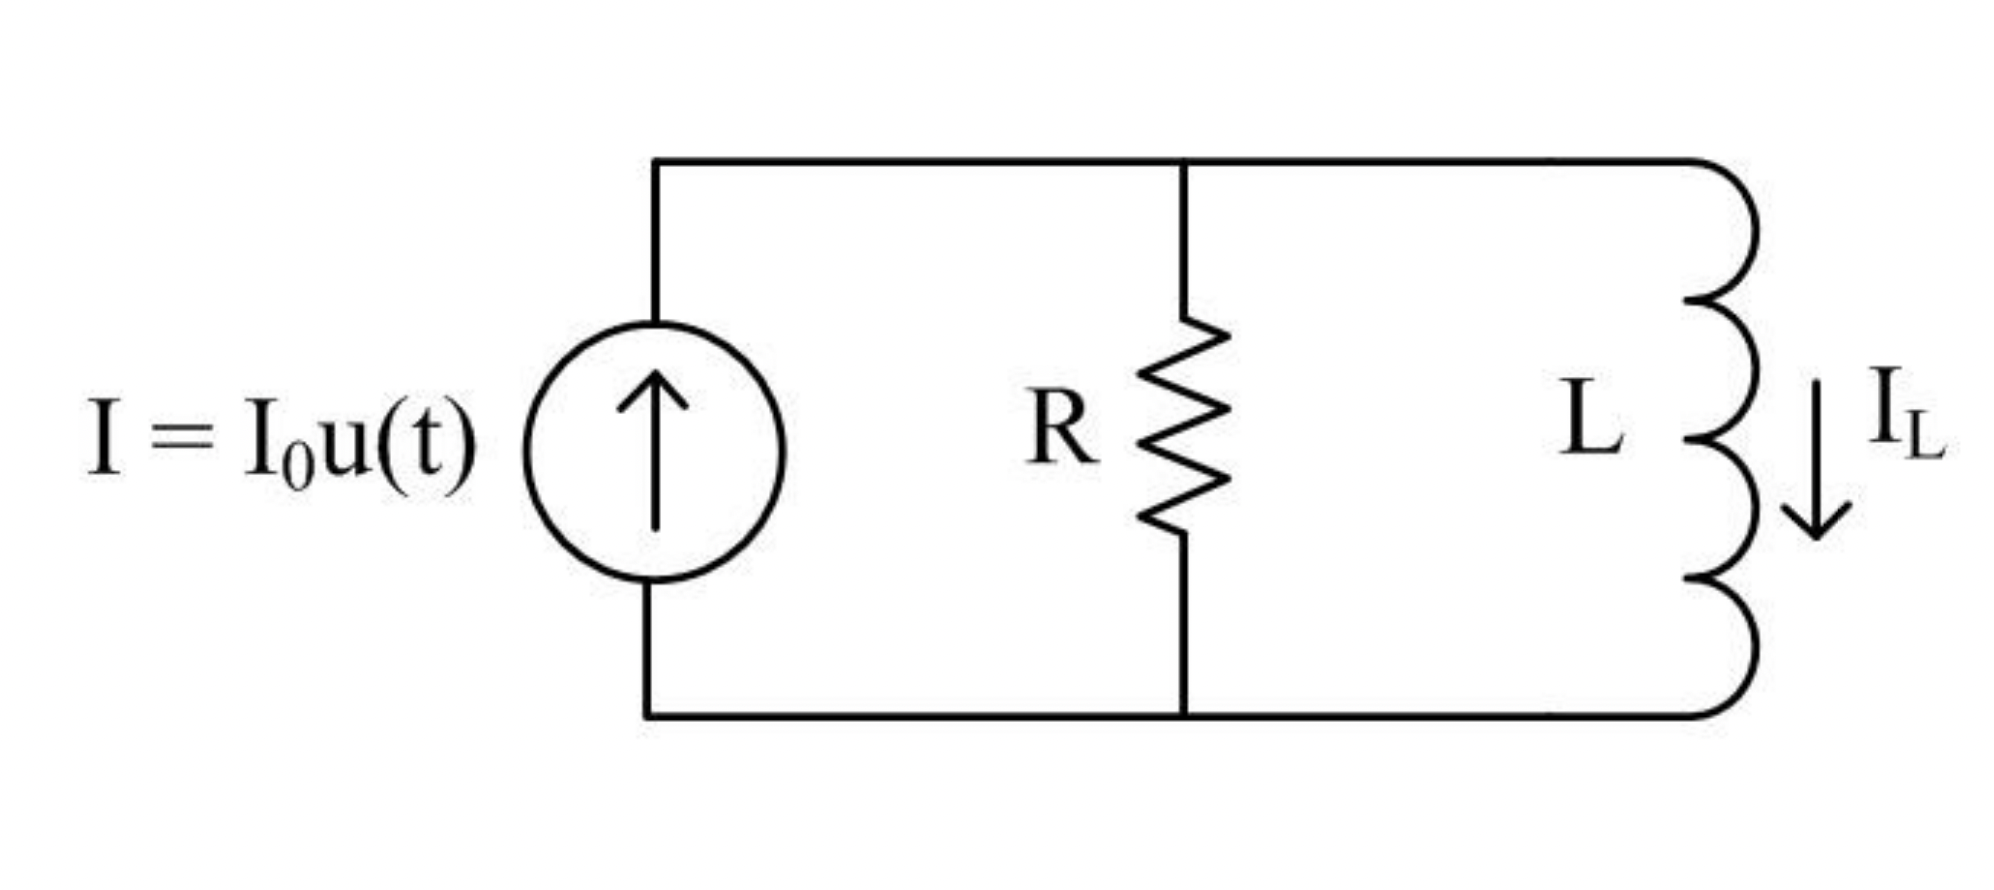
\includegraphics[width=\columnwidth]{2023/IN/43/figs/question.png}
\end{figure}\\
\renewcommand{\labelenumi}{\alph{enumi})}
\begin{enumerate}
\item $\frac{10000}{s^2+2s+10000}$\\
\item $\frac{10000}{s^2+2s+10000}e^{-0.05s}$\\
\item $\frac{10000}{s^2+2s+10000}e^{-0.5\times10^{-12}s}$\\
\item $\frac{100}{s^2+2s+100}$
\end{enumerate}
\hfill{(GATE IN 2023)}
\\\\
\solution
\fi
Drawing bode plots for four options.\\
\begin{align}
\implies H\brak{s}=\frac{k}{s ^{2}+2s+k}e^{as}\\
H\brak{j\omega}=\frac{k}{k-\omega ^2+2j\omega}e^{aj\omega}\\
\abs{H\brak{j\omega}}=\frac{k}{\sqrt{\brak{k-\omega ^2}^2+4\omega^2}}\\
\implies \phi\brak{H\brak{j\omega}}=\brak{-\tan^{-1}{\brak{\frac{2\omega}{k-\omega^2}}-a\omega}}
\end{align}
From the graphs , the answer is b

\begin{figure}[h]
    \centering
    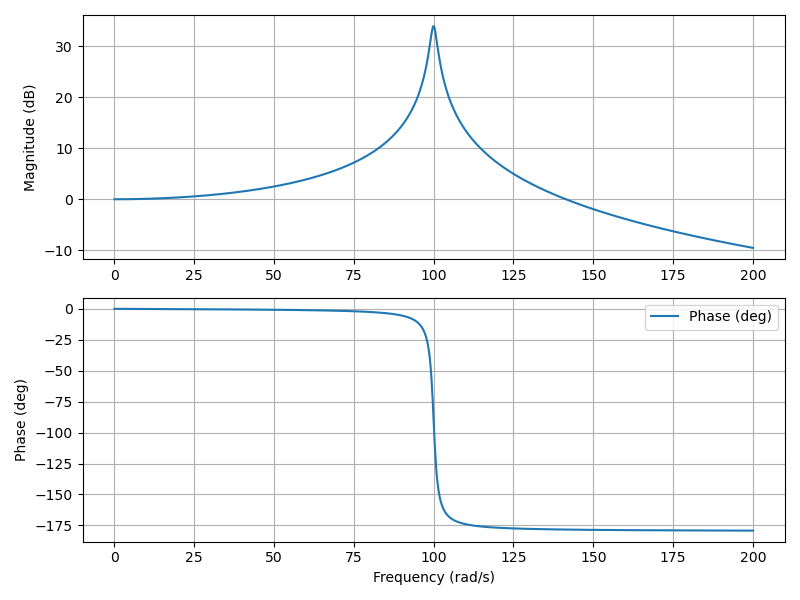
\includegraphics[width=\linewidth]{2023/IN/43/figs/A.png}
    \caption{Bode plot of a $\frac{10000}{s^2+2s+10000}$}
\end{figure}
\begin{figure}[h]
    \centering
    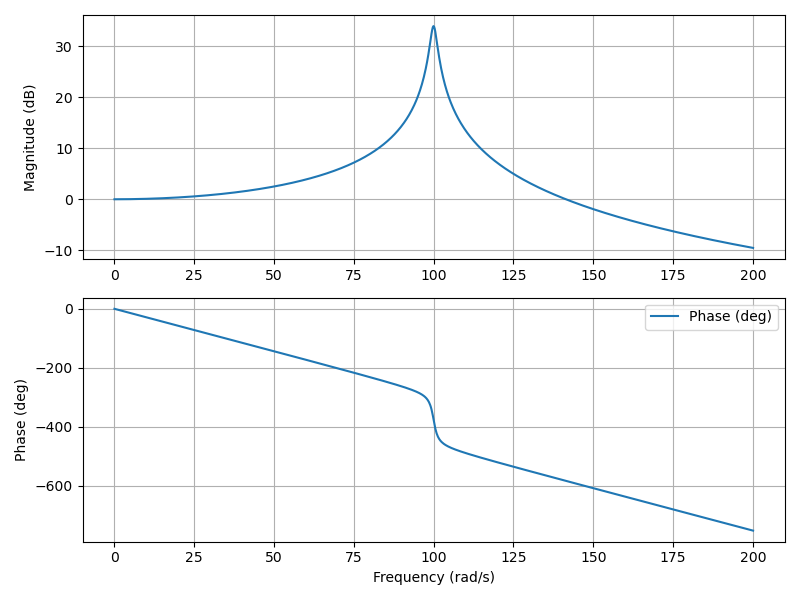
\includegraphics[width=\linewidth]{2023/IN/43/figs/B.png}
    \caption{Bode plot of a $\frac{10000e^{-0.05s}}{s^2+2s+10000}$}
\end{figure}
\begin{figure}[h]
    \centering
    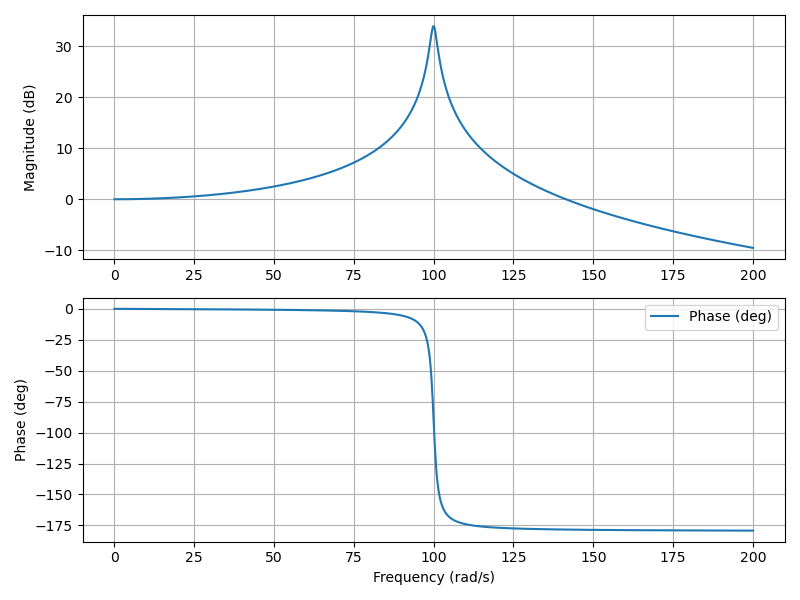
\includegraphics[width=\linewidth]{2023/IN/43/figs/C.png}
    \caption{Bode plot of a $\frac{10000e^{0.5\times10^{-12}s}}{s^2+2s+10000}$}
\end{figure}
\begin{figure}[h]
    \centering
    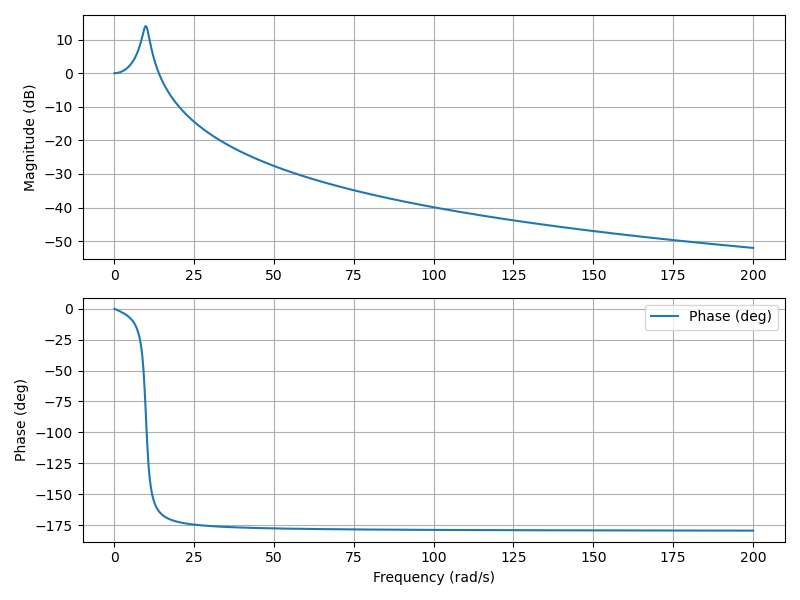
\includegraphics[width=\linewidth]{2023/IN/43/figs/D.png}
    \caption{Bode plot of a $\frac{100}{s^2+2s+100}$}
\end{figure}
%\end{document}

\newpage
\item The Laplace transform of the continuous-time signal $x\brak{t} = e^{-3t}u\brak{t - 5}$ is 
\rule{1cm}{0.15mm}, where $u\brak{t}$ denotes the continuous-time unit step signal.

\begin{enumerate}[label = \Alph*)]
    \item $\frac{e^{-5s}}{s + 3}$, Real$\{s\} > -3$\\
    \item $\frac{e^{-5(s - 3)}}{s - 3}$, Real$\{s\} > 3$\\
    \item $\frac{e^{-5(s + 3)}}{s + 3}$, Real$\{s\} > -3$\\
    \item $\frac{e^{-5(s - 3)}}{s + 3}$, Real$\{s\} > -3$\\
\end{enumerate}
\solution
\iffalse
\let\negmedspace\undefined
\let\negthickspace\undefined
\documentclass[journal,12pt,twocolumn]{IEEEtran}
\usepackage{cite}
\usepackage{amsmath,amssymb,amsfonts}
\usepackage{graphicx}
\usepackage{textcomp}
\usepackage{xcolor}
\usepackage{txfonts}
\usepackage{listings}
\usepackage{enumitem}
\usepackage{mathtools}
\usepackage{gensymb}
\usepackage{comment}
\usepackage[breaklinks=true]{hyperref}
\usepackage{tkz-euclide} 
\usepackage{listings}
\usepackage{gvv}                                        
\def\inputGnumericTable{}                                 
\usepackage[latin1]{inputenc}                                
\usepackage{color}                                            
\usepackage{array}                                            
\usepackage{longtable}                                       
\usepackage{calc}                                             
\usepackage{multirow}                                         
\usepackage{hhline}                                           
\usepackage{ifthen}                                           
\usepackage{lscape}
\usepackage[export]{adjustbox}

\newtheorem{theorem}{Theorem}[section]
\newtheorem{problem}{Problem}
\newtheorem{proposition}{Proposition}[section]
\newtheorem{lemma}{Lemma}[section]
\newtheorem{corollary}[theorem]{Corollary}
\newtheorem{example}{Example}[section]
\newtheorem{definition}[problem]{Definition}
\newcommand{\BEQA}{\begin{eqnarray}}
\newcommand{\EEQA}{\end{eqnarray}}
\newcommand{\define}{\stackrel{\triangle}{=}}
\newtheorem{rem}{Remark}

\begin{document}
\parindent 0px
\bibliographystyle{IEEEtran}

\vspace{3cm}

\title{}
\author{EE23BTECH11042 -  Khusinadha Naik$^{*}$
}
\maketitle
\newpage
\bigskip

% \renewcommand{\thefigure}{\theenumi}
% \renewcommand{\thetable}{\theenumi}


\noindent \textbf{26.} \hspace{2pt}A causal, discrete time system is described by the difference equation $y[n] = 0.5 y[n-1] + x[n]$, for all $n$, where $y[n]$ denotes the output sequence and $x[n]$ denotes the input sequence. Which of the following statements is/are TRUE?
\begin{flushright}
\hfill(GATE 2023 BM)
\end{flushright}
\begin{enumerate}[label = (\alph*)]
	\item The system has an impulse response described by $0.5^{n} u[-n]$ where $u[n]$ is the  
unit step sequence. 	\label{option:GATE.2023.BM.26.1}	
	\item The system is stable in the bounded input, bounded output sense.		\label{option:GATE.2023.BM.26.2}
	\item The system has an infinite number of non-zero samples in its impulse response	\label{option:GATE.2023.BM.26.3}
	\item The system has a finite number of non-zero samples in its impulse response.	\label{option:GATE.2023.BM.26.4}
\end{enumerate}

\noindent \textbf{Ans.}\\
\fi
\begin{table}[h]
\centering
\begin{tabular}{|c|c|c|}
        \hline
        \textbf{Parameter} & \textbf{Value} & \textbf{Description} \\
        \hline
        $x[n]$ & ? & Input Sequence \\
        \hline
        $y[n]$ & ? & Output Sequence \\
        \hline
\end{tabular}
\caption{Input parameters table}
\label{tab:GATE.2023.BM.26.1}





\end{table}
\begin{align}
y[n] = 0.5y[n-1] + x[n] 
\end{align}

Taking $Z$-Transform 
\begin{align}
Y\brak{z} &= 0.5z^{-1}Y\brak{z} + X\brak{z} \\
\implies \frac{Y\brak{z}}{X\brak{z}} &= \frac{1}{1 - 0.5z^{-1}} = H\brak{z} 
\end{align}
If $x[n]$ is impulse input 
\begin{align}
\implies &Y\brak{z} = H\brak{z} = \frac{1}{1 - 0.5z^{-1}}  \label{eq:GATE.2023.BM.26.4}
\end{align}
From \eqref{eq:GATE.2023.BM.26.4} pole lies at $z = 0.5$
\begin{align}
a^{n}u\brak{n} \xleftrightarrow{\mathcal{Z}} &\frac{1}{1 - az^{-1}} \quad , \abs{z} > a \label{eq:GATE.2023.BM.26.5}
\end{align}

From \eqref{eq:GATE.2023.BM.26.4} , \eqref{eq:GATE.2023.BM.26.5}
\begin{align}
h[n] = 0.5^{n}u[n] \quad , \abs{z} > 0.5 \label{eq:GATE.2023.BM.26.6}
\end{align}


\pagebreak
Plotting $h[n]$ vs $n$
\begin{figure}[h]
    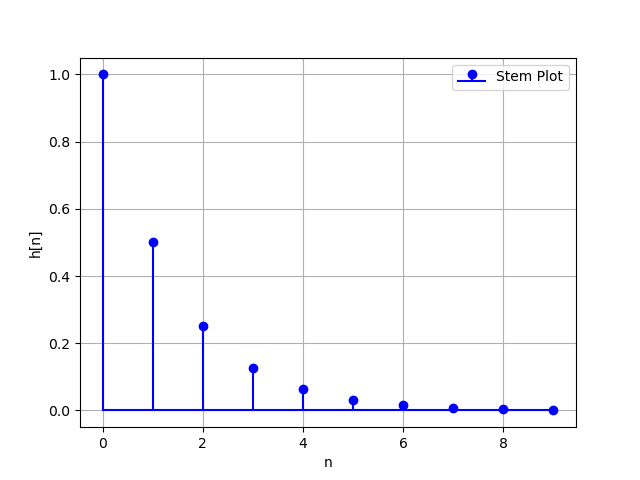
\includegraphics[width=0.5\textwidth]{2023/BM/26/figs/fig1.png}
    \caption{Plot of $h[n]$ vs $n$}
    \label{fig:GATE.2023.BM.26.1}
\end{figure}

\begin{enumerate}
\item From \eqref{eq:GATE.2023.BM.26.6} , \ref{option:GATE.2023.BM.26.1} is wrong
\item As pole lies within unit circle \ref{option:GATE.2023.BM.26.2} is true
\item From \eqref{eq:GATE.2023.BM.26.6} and \figref{fig:GATE.2023.BM.26.1} ,\ref{option:GATE.2023.BM.26.3} is true and hence
\item \ref{option:GATE.2023.BM.26.4} is false 
\end{enumerate}





%\end{document}


\newpage

\item The solution $x\brak{t}$, $t \geq 0$, to the differential equation
$\ddot{x} = -k\dot{x} , k > 0$ with initial conditions $x\brak{0} = 1$ and $\dot{x}\brak{0} = 0$ is
\begin{enumerate}[label = (\Alph*)]
    \item $x\brak{t} = 2e^{-kt} + 2kt -1 $\label{gate.in.20.a} \\
    \item $x\brak{t} = 2e^{-kt} -1 $\label{gate.in.20.b}\\
    \item $x\brak{t} = 1 $\label{gate.in.20.c}\\
    \item $x\brak{t} = 2e^{-kt} - kt - 1 $\label{gate.in.20.d}
\end{enumerate}
\hfill{GATE ~2023  , IN}\\
\solution
\iffalse
\let\negmedspace\undefined
\let\negthickspace\undefined
\documentclass[journal,12pt,twocolumn]{IEEEtran}
\usepackage{cite}
\usepackage{amsmath,amssymb,amsfonts,amsthm}
\usepackage{algorithmic}
\usepackage{graphicx}
\usepackage{textcomp}
\usepackage{xcolor}
\usepackage{txfonts}
\usepackage{listings}
\usepackage{enumitem}
\usepackage{mathtools}
\usepackage{gensymb}
\usepackage{comment}
\usepackage[breaklinks=true]{hyperref}
\usepackage{tkz-euclide} 
\usepackage{listings}
\usepackage{gvv}                                        
\def\inputGnumericTable{}                                 
\usepackage[latin1]{inputenc}                                
\usepackage{color}                                            
\usepackage{array}                                            
\usepackage{longtable}                                       
\usepackage{calc}                                             
\usepackage{multirow}                                         
\usepackage{hhline}                                           
\usepackage{ifthen}                                           
\usepackage{lscape}

\newtheorem{theorem}{Theorem}[section]
\newtheorem{problem}{Problem}
\newtheorem{proposition}{Proposition}[section]
\newtheorem{lemma}{Lemma}[section]
\newtheorem{corollary}[theorem]{Corollary}
\newtheorem{example}{Example}[section]
\newtheorem{definition}[problem]{Definition}
\newcommand{\BEQA}{\begin{eqnarray}}
\newcommand{\EEQA}{\end{eqnarray}}
\newcommand{\define}{\stackrel{\triangle}{=}}
\theoremstyle{remark}
\newtheorem{rem}{Remark}

\usepackage{graphicx}
\graphicspath{ {./Downloads/} }
\begin{document}

\bibliographystyle{IEEEtran}
\vspace{3cm}

\title{GATE 2023}
\author{EE22BTECH11060 - TEJAVATH KUSHAL$^{*}$% <-this % stops a space
}
\maketitle
\newpage
\bigskip

\renewcommand{\thefigure}{\theenumi}
\renewcommand{\thetable}{\theenumi}

\maketitle
\noindent \textbf{Q 20 :} The solution \(x(t)\), \(t \geq 0\), to the differential equation
$\ddot{x} = -k\dot{x} , k > 0$
with initial conditions \(x(0) = 1\) and \(\dot{x} (0) = 0\) is: 
\begin{enumerate}[label = (\Alph*)]
    \item $x\brak{t}$ = 2e^{-kt} + 2kt -1 \label{gate.in.20.a}\\
    \item $x\brak{t}$ = 2e^{-kt} -1 \label{gate.in.20.b}\\
    \item $x\brak{t}$ = 1 \label{gate.in.20.c}\\
    \item $x\brak{t}$ = 2e^{-kt} - kt - 1 \label{gate.in.20.d}
\end{enumerate}
\hfill{GATE ~2023  , IN} 
\\
\noindent \textbf{Ans}:\\ \\
\fi
\begin{table}[h]
\centering
\begin{tabular}{ | c | c|  } 
  \hline
   Differential equation & $\ddot{x} = -k\dot{x}$ \\ 
  \hline
  Initial conditions & $x\brak{0}=1$ and $\dot{x}\brak{0}=0$ \\
  \hline
  $x\brak{t}$ & $?$ \\ 
  \hline
 
\end{tabular}
\caption{Parameter Table}
\label{tab:gate2023.in.20.1}

\end{table}
\begin{align}
    \implies \frac{d^2 x(t)}{dt^2} = -k\frac{dx(t)}{dt}
\end{align}\\

Taking Laplace transform on both sides,\\
\begin{align}
\label{eq:gate2023.in.20.2}\frac{d^2x\brak{t}}{dx^2} &\system{L}
       s^2X(s)-sx(0)-\dot{x}(0)\\
\label{eq:gate2023.in.20.3}\frac{dx\brak{t}}{dx} &\system{L} sX(s)-x(0)
\end{align}

From Table \eqref{eq:gate2023.in.20.2} , \eqref{eq:gate2023.in.20.3} 
\begin{align}
s^2 X\brak{s} - sx\brak{0} - \dot{x}\brak{0} &= -k\brak{sX\brak{s} - x\brak{0}} \\
s^2 X\brak{s} - s &= -k\brak{sX\brak{s}-1} \\
sX\brak{s}\brak{s+k}&=\brak{s+k}\\
     X\brak{s}&=\frac{1}{s} \quad , s \neq -k \\
     x\brak{t}&=u\brak{t}\\
      \implies x\brak{t}&=1 \quad \brak{t\geq 0}
\end{align}\\
Thus, the correct option is \ref{gate.in.20.c}
%\pagebreak
\begin{figure}[h]
    %\caption{ Plot of $x\brak{t}$ v/s t}
    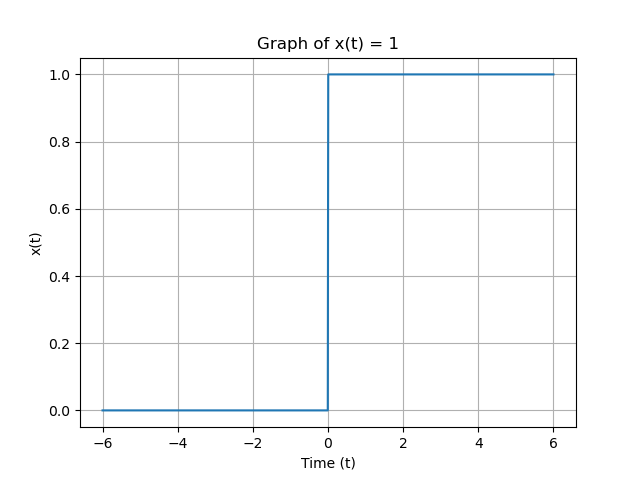
\includegraphics[width=0.5\textwidth]{2023/IN/20/figs/x(t)_vs_t.png}
    \caption{Plot of $x\brak{t}$ v/s t}
\end{figure}


\pagebreak
\item  Consider the differential equation
\begin{align}
x^2\frac{d^2y}{dx^2} + 4x\frac{dy}{dx} + 2y = 0 \quad \text{for } x\geq 1 \nonumber
\end{align}
with initial conditions $y=0$ and $\frac{dy}{dx} = 1$ at
$x = 1$. The value of $y$ at $x = 2$ is ?\\

\hfill(GATE AE 54 2023)\\
\solution
\iffalse
\let\negmedspace\undefined
\let\negthickspace\undefined
\documentclass[journal,12pt,twocolumn]{IEEEtran}
\usepackage{cite}
\usepackage{amsmath,amssymb,amsfonts}
\usepackage{graphicx}
\usepackage{textcomp}
\usepackage{xcolor}
\usepackage{txfonts}
\usepackage{listings}
\usepackage{enumitem}
\usepackage{mathtools}
\usepackage{gensymb}
\usepackage{comment}
\usepackage[breaklinks=true]{hyperref}
\usepackage{tkz-euclide} 
\usepackage{listings}
\usepackage{gvv}                                        
\def\inputGnumericTable{}                                 
\usepackage[latin1]{inputenc}                                
\usepackage{color}                                            
\usepackage{array}                                            
\usepackage{longtable}                                       
\usepackage{calc}                                             
\usepackage{multirow}                                         
\usepackage{hhline}                                           
\usepackage{ifthen}                                           
\usepackage{lscape}
\usepackage[export]{adjustbox}

\newtheorem{theorem}{Theorem}[section]
\newtheorem{problem}{Problem}
\newtheorem{proposition}{Proposition}[section]
\newtheorem{lemma}{Lemma}[section]
\newtheorem{corollary}[theorem]{Corollary}
\newtheorem{example}{Example}[section]
\newtheorem{definition}[problem]{Definition}
\newcommand{\BEQA}{\begin{eqnarray}}
\newcommand{\EEQA}{\end{eqnarray}}
\newcommand{\define}{\stackrel{\triangle}{=}}
\newtheorem{rem}{Remark}

\begin{document}
\parindent 0px
\bibliographystyle{IEEEtran}

\vspace{3cm}

\title{}
\author{EE23BTECH11042 -  Khusinadha Naik$^{*}$
}
\maketitle
\newpage
\bigskip

% \renewcommand{\thefigure}{\theenumi}
% \renewcommand{\thetable}{\theenumi}


\noindent \textbf{26.} \hspace{2pt}A causal, discrete time system is described by the difference equation $y[n] = 0.5 y[n-1] + x[n]$, for all $n$, where $y[n]$ denotes the output sequence and $x[n]$ denotes the input sequence. Which of the following statements is/are TRUE?
\begin{flushright}
\hfill(GATE 2023 BM)
\end{flushright}
\begin{enumerate}[label = (\alph*)]
	\item The system has an impulse response described by $0.5^{n} u[-n]$ where $u[n]$ is the  
unit step sequence. 	\label{option:GATE.2023.BM.26.1}	
	\item The system is stable in the bounded input, bounded output sense.		\label{option:GATE.2023.BM.26.2}
	\item The system has an infinite number of non-zero samples in its impulse response	\label{option:GATE.2023.BM.26.3}
	\item The system has a finite number of non-zero samples in its impulse response.	\label{option:GATE.2023.BM.26.4}
\end{enumerate}

\noindent \textbf{Ans.}\\
\fi
\begin{table}[h]
\centering
\begin{tabular}{|c|c|c|}
        \hline
        \textbf{Parameter} & \textbf{Value} & \textbf{Description} \\
        \hline
        $x[n]$ & ? & Input Sequence \\
        \hline
        $y[n]$ & ? & Output Sequence \\
        \hline
\end{tabular}
\caption{Input parameters table}
\label{tab:GATE.2023.BM.26.1}





\end{table}
\begin{align}
y[n] = 0.5y[n-1] + x[n] 
\end{align}

Taking $Z$-Transform 
\begin{align}
Y\brak{z} &= 0.5z^{-1}Y\brak{z} + X\brak{z} \\
\implies \frac{Y\brak{z}}{X\brak{z}} &= \frac{1}{1 - 0.5z^{-1}} = H\brak{z} 
\end{align}
If $x[n]$ is impulse input 
\begin{align}
\implies &Y\brak{z} = H\brak{z} = \frac{1}{1 - 0.5z^{-1}}  \label{eq:GATE.2023.BM.26.4}
\end{align}
From \eqref{eq:GATE.2023.BM.26.4} pole lies at $z = 0.5$
\begin{align}
a^{n}u\brak{n} \xleftrightarrow{\mathcal{Z}} &\frac{1}{1 - az^{-1}} \quad , \abs{z} > a \label{eq:GATE.2023.BM.26.5}
\end{align}

From \eqref{eq:GATE.2023.BM.26.4} , \eqref{eq:GATE.2023.BM.26.5}
\begin{align}
h[n] = 0.5^{n}u[n] \quad , \abs{z} > 0.5 \label{eq:GATE.2023.BM.26.6}
\end{align}


\pagebreak
Plotting $h[n]$ vs $n$
\begin{figure}[h]
    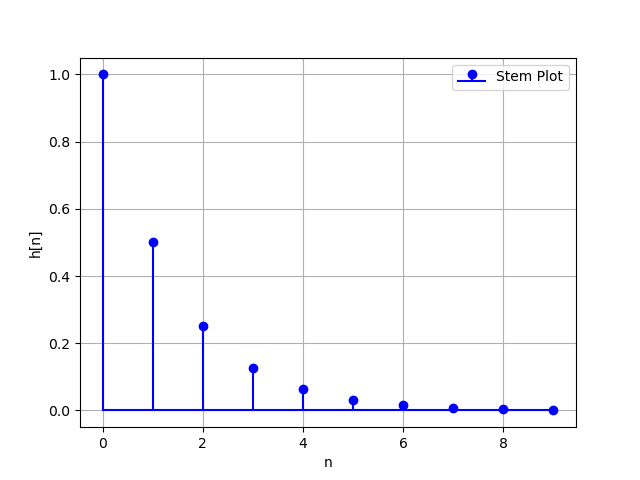
\includegraphics[width=0.5\textwidth]{2023/BM/26/figs/fig1.png}
    \caption{Plot of $h[n]$ vs $n$}
    \label{fig:GATE.2023.BM.26.1}
\end{figure}

\begin{enumerate}
\item From \eqref{eq:GATE.2023.BM.26.6} , \ref{option:GATE.2023.BM.26.1} is wrong
\item As pole lies within unit circle \ref{option:GATE.2023.BM.26.2} is true
\item From \eqref{eq:GATE.2023.BM.26.6} and \figref{fig:GATE.2023.BM.26.1} ,\ref{option:GATE.2023.BM.26.3} is true and hence
\item \ref{option:GATE.2023.BM.26.4} is false 
\end{enumerate}





%\end{document}

\pagebreak

\item Consider a lead compensator of the form \\
$K(s) = \frac{1 + \frac{s}{a}}{1 + \frac{s}{\beta a}}, \quad \beta > 1, \quad a > 0$\\
The frequency at which this compensator produces maximum phase lead is \(4 \, \text{rad/s}\). At this frequency, the gain amplification provided by the controller, assuming an asymptotic Bode-magnitude plot of \(K(s)\), is \(6 \, \text{dB}\). The values of \(a\) and \(\beta\), respectively, are
\begin{enumerate}
    \item $ 1, 16 $\\
    \item $\ 2, 4 $\\
    \item $ 3, 5 $\\
    \item $ 2.66, 2.25$\\
\end{enumerate}\hfill{(GATE EE 2023)}
\solution
\input{2023/EE/38/38.tex}
\newpage

\item Second order ordinary differential equation $\frac{d^2y}{dx^2}-\frac{dy}{dx}-2y=0$ has values 
$y=2$ and$\frac{dy}{dx}=1$ at $x=0$.The value of $y$ at $x=1$ is?($round\; off\;\: to\;\: three\;\: decimal\;\: places$)
 \\ \hfill[GATE-ES 2023]\\
 \solution
  \input{2023/ES/47/gate[es.47].tex}
 \newpage

 \item A continuous-time system that is initially at rest is described by,	
	\begin{center}
		$\dfrac{dy(t)}{dt} + 3y(t) = 2x(t)$
	\end{center}
where $x(t)$ is the input voltage and $y(t)$ is the output voltage.\\ 
The impulse response of the system is?
\hfill(GATE EE 2023)
\solution
\iffalse
\let\negmedspace\undefined
\let\negthickspace\undefined
\documentclass[journal,12pt,onecolumn]{IEEEtran}
\usepackage{cite}
\usepackage{amsmath,amssymb,amsfonts,amsthm}
\usepackage{algorithmic}
\usepackage{graphicx}
\usepackage{textcomp}
\usepackage{xcolor}
\usepackage{txfonts}
\usepackage{listings}
\usepackage{enumitem}
\usepackage{mathtools}
\usepackage{gensymb}
\usepackage{comment}
\usepackage[breaklinks=true]{hyperref}
\usepackage{tkz-euclide} 
\usepackage{listings}
\usepackage{gvv}                                        
\def\inputGnumericTable{}                                 
\usepackage[latin1]{inputenc}                                
\usepackage{color}                                            
\usepackage{array}                                            
\usepackage{longtable}                                       
\usepackage{calc}                                             
\usepackage{multirow}                                         
\usepackage{hhline}                                           
\usepackage{ifthen}                                           
\usepackage{lscape}
\usepackage{siunitx}
\usepackage{flushend}
\usepackage[siunitx]{circuitikz}
\usepackage{caption}

\newtheorem{theorem}{Theorem}[section]
\newtheorem{problem}{Problem}
\newtheorem{proposition}{Proposition}[section]
\newtheorem{lemma}{Lemma}[section]
\newtheorem{corollary}[theorem]{Corollary}
\newtheorem{example}{Example}[section]
\newtheorem{definition}[problem]{Definition}
\newcommand{\BEQA}{\begin{eqnarray}}
	\newcommand{\EEQA}{\end{eqnarray}}
\newcommand{\define}{\stackrel{\triangle}{=}}
\theoremstyle{remark}
\newtheorem{rem}{Remark}
\begin{document}
	
	\bibliographystyle{IEEEtran}
	\vspace{3cm}
	
	\title{GATE EE Q.17}
	\author{EE23BTECH11203 - Adarsh A$^{*}$% <-this % stops a space
	}
	\maketitle
	%\newpage
	\bigskip
	
	\renewcommand{\thefigure}{\theenumi}
	\renewcommand{\thetable}{\theenumi}
	
	
	\vspace{0.2cm}
	\linespread{1.1}
	
	
	\textbf{ Question : }
	 A continuous-time system that is initially at rest is described by,
	\begin{center}
		$\dfrac{dy(t)}{dt} + 3y(t) = 2x(t)$
	\end{center}
	where $x(t)$ is the input voltage and $y(t)$ is the output voltage.\\ 
	The impulse response of the system is?
	
	\vspace{0.2cm}
	
	(A) 3$e^{-2t}$
	
	\vspace{0.3cm}
	
	(B) $\dfrac{1}{3}e^{-2t} u(t)$
	
	\vspace{0.3cm}
	
	(C) 2$e^{-3t} u(t)$
	
	\vspace{0.2cm}
	
	(D) 2$e^{-3t}$ \hfill(GATE 2023 EE)
	
	\vspace{0.2cm}
	
	\solution
	
	\begin{table}[htbp]
	\centering
	\noindent
	\fontsize{10}{15}\selectfont {
		\resizebox{0.45\textwidth}{!}{%
			\begin{tabular}{|c|c|c|}
				\hline
				\textbf{Parameter} & \textbf{Value} & \textbf{Description} \\
				\hline
				$x\brak t$ & - & Input voltage \\
				\hline
				$y\brak t$ & - & Output voltage \\
				\hline
				$h\brak t$ & $\frac{y\brak t}{x\brak t}$ & Impulse response \\
				\hline
				$X\brak s$ & - & Input voltage in s-domain \\
				\hline
				$Y\brak s$ & - & Output voltage in s-domain \\
				\hline
				$H\brak s$ & $\frac{Y\brak s}{X\brak s}$ & Impulse response in s-domain \\
				\hline
			\end{tabular}
	} }
	\caption*{Input Table}
	
\end{table}
	\fi
	%\vspace{-0.3cm}
	
	Given equation is,
	\begin{align}
		\dfrac{dy(t)}{dt} + 3y(t) &= 2x(t)
	\end{align}
	
	Applying Laplace transform,
	\begin{align}
		x\brak{t} &
		\xleftarrow[]{\hspace{0.4cm}{\mathcal{L}}\hspace{0.1cm}}\xrightarrow[]{}
		X\brak{s}\\
		y\brak{t} &
		\xleftarrow[]{\hspace{0.4cm}{\mathcal{L}}\hspace{0.1cm}}\xrightarrow[]{}
		Y\brak{s}
	\end{align}
	
	
	%\vspace{0.5cm}
	
	From the differentiation property,
	
	\begin{align}
		\dfrac{dy\brak t}{dt} &
		\xleftarrow[]{\hspace{0.4cm}{\mathcal{L}}\hspace{0.1cm}}\xrightarrow[]{}
		s Y\brak{s}
	\end{align}
	%\vspace{0.4cm}
	The equation becomes,
	\begin{align}
		s Y\brak s + 3 Y\brak s &= 2 X\brak s\\
		Y\brak s \brak {s + 3} &= 2 X\brak s\\[5pt]
		H\brak s &= \dfrac{Y\brak s}{X\brak s}\\[5pt]
		H\brak s &= \dfrac{2}{s + 3}
	\end{align}
	\begin{align}
		\dfrac{1}{s + a} &
		\xleftarrow[]{\hspace{0.4cm}{\mathcal{L}}\hspace{0.1cm}}\xrightarrow[]{}
		e^{-at} u\brak t
	\end{align}
	
	Using these results,
	\begin{align}
		h\brak t &= 2 e^{-3t} u\brak t 
	\end{align}
	
	%\vspace{0.2cm}
	
	%\underline{Plot of $h\brak t$ $vs$ $t$} :
	
	\begin{figure}[htbp]
		\centering
		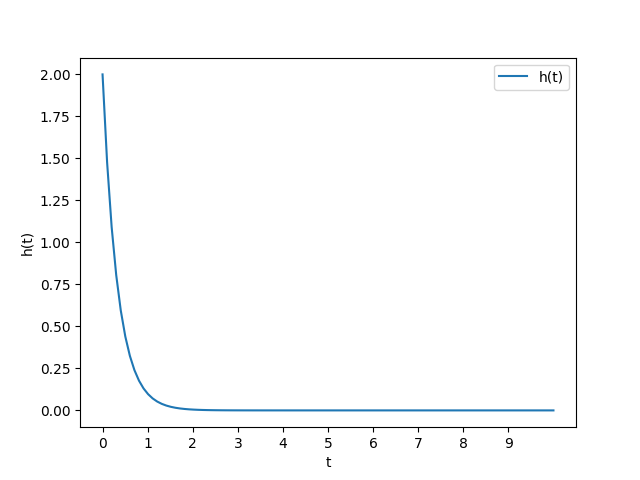
\includegraphics[width=0.6\textwidth]{figs/figure1.png}
		\caption*{(a) Plot of $h\brak t$ $vs$ $t$}
	\end{figure}
	
%\end{document}

\newpage

\item Consider the equation $\frac{dy}{dx}+ay=\sin{\omega x}$,where $a$ and $\omega$ are constants.Given $y=1$ at $x=0$, correct all the correct statement(s) from the following as $x\to \infty$.
\begin{enumerate}

  \item[(A)]  $y \to 0$ if $a \neq 0$ \\ 
  \item[(B)]  $y \to 1$ if $a = 0$\\
  \item[(C)]  $y \to Aexp(|a|x)$ if $a < 0$; A is constant\\
  \item[(D)]  $y \to B \sin(\omega x+C)$ if $a>0$; B and C are constants\\
\end{enumerate}
\hfill(GATE AE 2023)
\solution
\input{2023/AE/42/assignment3.tex}
\newpage


\item \textbf{Question }:
The position $x(t)$ of a particle, at constant $\omega$, is described by the equation
\begin{align}
\frac{{d^2x}}{{dt^2}} = -\omega^2 x.
\end{align}
The initial conditions are $x(t=0)=1$ and $\frac{{dx}}{{dt}}\bigg|_{t=0}=0$. 
The position of the particle at $t=\frac{{3\pi}}{{\omega}}$ is \underline{\hspace{2cm}} (in integer).
\hfill{(GATE CH 2023)}
\solution
% \iffalse
\let\negmedspace\undefined
\let\negthickspace\undefined
\documentclass[journal,12pt,twocolumn]{IEEEtran}
\usepackage{cite}
\usepackage{amsmath,amssymb,amsfonts,amsthm}
\usepackage{algorithmic}
\usepackage{graphicx}
\usepackage{textcomp}
\usepackage{xcolor}
\usepackage{txfonts}
\usepackage{listings}
\usepackage{enumitem}
\usepackage{mathtools}
\usepackage{gensymb}
\usepackage{comment}
\usepackage[breaklinks=true]{hyperref}
\usepackage{tkz-euclide} 
\usepackage{listings}
\usepackage{gvv}  
\usepackage{tikz}
\usepackage{circuitikz} 
\usepackage{caption}

\def\inputGnumericTable{}                                
\usepackage[latin1]{inputenc}                 
\usepackage{color}                            
\usepackage{array}                            
\usepackage{longtable}                        
\usepackage{calc}                            
\usepackage{multirow}                      
\usepackage{hhline}                           
\usepackage{ifthen}                          
\usepackage{lscape}
\usepackage{amsmath}
\newtheorem{theorem}{Theorem}[section]
\newtheorem{problem}{Problem}
\newtheorem{proposition}{Proposition}[section]
\newtheorem{lemma}{Lemma}[section]
\newtheorem{corollary}[theorem]{Corollary}
\newtheorem{example}{Example}[section]
\newtheorem{definition}[problem]{Definition}
\newcommand{\BEQA}{\begin{eqnarray}}
\newcommand{\EEQA}{\end{eqnarray}}
\newcommand{\define}{\stackrel{\triangle}{=}}
\theoremstyle{remark}
\newtheorem{rem}{Remark}

\begin{document}
\title{Gate Assignment CH 31}
\author{Shravya Kantayapalam\\ EE23BTECH11030}
\maketitle

\begin{enumerate}
    \item \textbf{Question }:
The position \( x(t) \) of a particle, at constant \( \omega \), is described by the equation
\[
\frac{{d^2x}}{{dt^2}} = -\omega^2 x.
\]
The initial conditions are \( x(t=0) = 1 \) and \( \frac{{dx}}{{dt}}\bigg|_{t=0} = 0 \). 

The position of the particle at \( t = \frac{{3\pi}}{{\omega}} \) is \underline{\hspace{2cm}} (in integer).
\hfill{(GATE CH 2023)}

\solution

\begin{table}[htbp]
    \centering
    \caption{Input Parameters}
    \begin{tabular}{|c|c|}
        \hline
        \textbf{Parameter} & \textbf{Description} \\
        \hline
        $s$ & Complex frequency variable in Laplace domain \\
        $\omega$ & Angular frequency \\
        $X(s)$ & Laplace transform of the function $x(t)$ \\
        $x(t)$ & Time-domain function \\
        \hline
    \end{tabular}
\end{table}

\[
s^2X(s) - sx(0) - \frac{{dx}}{{dt}}(0) + \omega^2X(s) = 0
\]

\[
x(0) = 1 \quad \text{and} \quad \frac{{dx}}{{dt}}(0) = 0
\]

\[
s^2X(s) - s - \omega^2X(s) = 0
\]

\[
(s^2 + \omega^2)X(s) = s
\]

\[
X(s) = \frac{{s}}{{s^2 + \omega^2}}
\]

\[
X(s) = \frac{{s}}{{s^2 + \omega^2}} = \frac{{A}}{{s}} + \frac{{Bs + C}}{{s^2 + \omega^2}}
\]

Multiplying both sides by $s(s^2 + \omega^2)$, we get:
\[
s = A(s^2 + \omega^2) + (Bs + C)s
\]

This implies $A = 0$, $B = 1$, and $C = 0$. Therefore,
\[
X(s) = \frac{{1}}{{s^2 + \omega^2}}
\]

\[
x(t) = \mathcal{L}^{-1} \left\{ \frac{{1}}{{s^2 + \omega^2}} \right\} = \cos(\omega t)
\]

Finally, evaluating $x(t)$ at $t = \frac{{3\pi}}{{\omega}}$, we have:
\[
x\left(\frac{{3\pi}}{{\omega}}\right) = \cos\left(\omega \cdot \frac{{3\pi}}{{\omega}}\right) = \cos(3\pi) = -1
\]
\begin{figure}[ht]
    \centering
    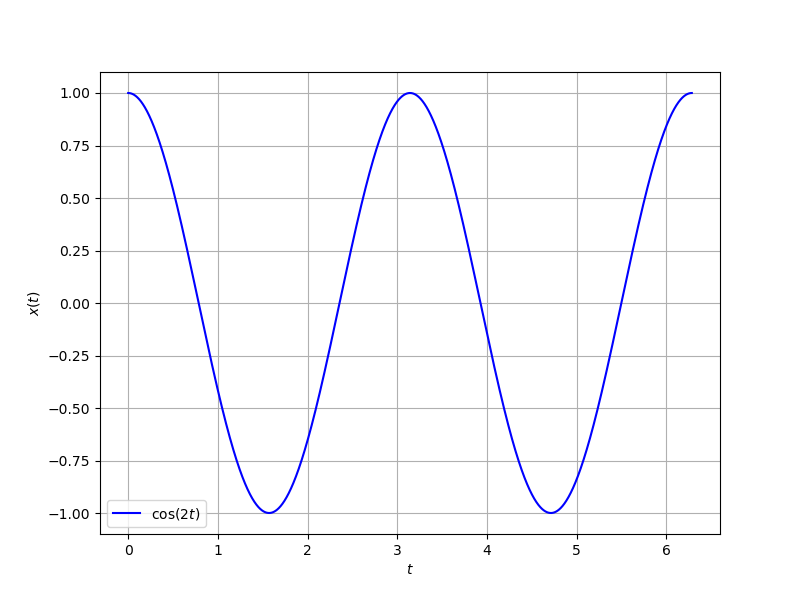
\includegraphics[width=\columnwidth]{figs/gate.png}
    \caption{Graph of $x(t)$}
\end{figure}
\end{document}



\newpage

\item \textbf{Question}:The initial value problem
$\frac{dy}{dt}+2y=0, y(0)=1 $
is solved numerically using the forward Euler's method with a constant and positive time step of $\delta $.\\
Let $y_n$ represent the numerical solution obtained after $n$ steps. The condition $\abs{y_{n+1}} \leq \abs{y_n}$is satisfied if and only if $\delta$ does not exceed \\
\hfill{(GATE ME 2023)}\\
\solution 
\iffalse
\documentclass[journal,12pt,twocolumn]{IEEEtran}
\usepackage{amsmath,amsfonts,amssymb,float,gvv,graphicx,enumitem,array,esint}
\bibliographystyle{IEEEtran}
\vspace{3cm}
\title{GATE 2023-ME-50}
\author{Pragnidhved Reddy\\EE23BTECH11050}
\date{}
\parindent 0px
\begin{document}
\maketitle
\newpage
\bigskip
\textbf{Question GATE 23 ME 50:}\\
The initial value problem
$\frac{dy}{dt}+2y=0, y(0)=1 $
is solved numerically using the forward Euler's method with a constant and positive time step of $\delta $.\\
Let $y_n$ represent the numerical solution obtained after $n$ steps. The condition $\abs{y_{n+1}} \leq \abs{y_n}$is satisfied if and only if $\delta$ does not exceed\\
\solution \\
\fi
Numerical solution: -\\
By forward Euler's method formula 
\begin{align}
\label{eq:eq1_ME_50}
    y(n+1)=y(n)+\delta  f(x,y)
\end{align}
From question we get
\begin{align}
\label{eq:eq2_ME_50}
\frac{dy}{dx}=-2y=f(x,y)
\end{align}
From \eqref{eq:eq2_ME_50} in \eqref{eq:eq1_ME_50}
\begin{align}
y(n+1)-y(n)&=-2\delta y(n)\\
y(n+1)&=(1-2\delta)y(n)\\
y(n)&\overset{Z}\longleftrightarrow Y(z)\\
y(n+1)&\overset{Z}\longleftrightarrow zY(z)-y(0)\\
\implies zY(z)-y(0)&=(1-2\delta)Y(z)\\
Y(z)&=\frac{1}{z-1+2\delta}\\
\frac{1}{z-(1-2\delta)}&\overset{Z}\longleftrightarrow (1-2\delta)^{n}u(n)
\end{align}
For good approximation we choose $\delta$ = 0.4
\begin{align}
y(n)&=(0.2)^nu(n)
\end{align}
Now using the condition given in question
\begin{align}
|y(n+1)| \leq |y(n)|\\
|(1-2\delta)^2| \leq |1-2\delta|\\
|1-2\delta| \leq 1 \\
0 \leq \delta \leq 1
\end{align}
From this we can say that the maximum value of $\delta  $ is 1\\
Theoritical solution: -\\
By properties of Laplace transform: -
\begin{align}
\label{eq:eq8_ME_50}
Y(s)&=\mathcal{L}y(s)\\
\label{eq:eq9_ME_50}
\mathcal{L}y'&=sY(s)-y(0)
\end{align}
Given equation: -
\begin{align}
y'+2y&=0\\
\mathcal{L}(y'+2y)&=0
\end{align}
From \eqref{eq:eq8_ME_50} and \eqref{eq:eq9_ME_50}
\begin{align}
sY(s)-1+2Y(s)&=0\\
\frac{1}{s+2}&=Y(s)\\
y(t)&=\mathcal{L}^{-1}Y(s)\\
\implies y(t)&=\mathcal{L}^{-1}\left(\frac{1}{s+2}\right)\\
\mathcal{L}^{-1}\left(\frac{1}{s+k}\right)&=e^{-kt}u(t)\\
\implies y(t)&=e^{-2t}u(t) 
\end{align}
\begin{figure}[h!]
    \centering
    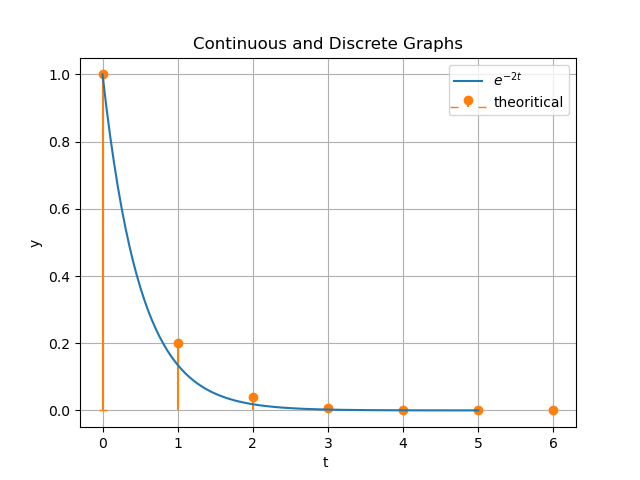
\includegraphics[width=\columnwidth]{2023/ME/50/figs/graph.png}
    \caption{simulation vs analysis}
\end{figure}



\newpage

\item In the context of signals and systems, determine the phase cross-over frequency of the open-loop transfer function
\[
G(s) = \frac{k \cdot s \cdot (1+sT_1) \cdot (1+sT_2)}{s}
\]
with positive constants $k, T_1, T_2$ are positive constants.The phase crossover fequency,in rad/s,is
\begin{enumerate}
  \item[(a)] $\frac{1}{\sqrt{T_1 T_2}}$
  \item[(b)] $\frac{1}{T_1 T_2}$
  \item[(c)] $\frac{1}{T_1\sqrt{T_2}}$
  \item[(d)] $\frac{1}{\sqrt{T_2}T_1}$
\end{enumerate}
\hfill{(GATE EC 2023)}\\
\solution
\iffalse
\documentclass[journal,12pt,twocolumn]{IEEEtran}
\usepackage{cite}
\usepackage{amsmath,amssymb,amsfonts,amsthm}
\usepackage{graphicx}
\title{GATE-2023 EC Q.25}
\author{EE23BTECH11214 - Harsha Vardhan Kumar}

\begin{document}
\maketitle

\textbf{Question}:
In the context of signals and systems, determine the phase cross-over frequency of the open-loop transfer function
\[
G(s) = \frac{k \cdot s \cdot (1+sT_1) \cdot (1+sT_2)}{s}
\]
with positive constants $k, T_1, T_2$ are positive constants.The phase crossover fequency,in rad/s,is
\hfill [EC,GATE-$2023$]
\begin{enumerate}
  \item[(a)] $\frac{1}{\sqrt{T_1 T_2}}$
  \item[(b)] $\frac{1}{T_1 T_2}$
  \item[(c)] $\frac{1}{T_1\sqrt{T_2}}$
  \item[(d)] $\frac{1}{\sqrt{T_2}T_1}$
\end{enumerate}
\textbf{Solution}:
\fi
The phase of \( G(s) \)
\begin{align}
\angle G(s) &= \angle (ks(1+sT_1)(1+sT_2)) - \angle s \\
&= \angle ks + \angle (1+sT_1) + \angle (1+sT_2) - \angle s 
\end{align}
The phase contribution of each term
\begin{align}
\angle ks &= \angle k + \angle s = 0 + \frac{\pi}{2} \\
&= \frac{\pi}{2} \text{ radians} \\
\angle (1+sT_1) &= \tan^{-1}(0) + \tan^{-1}(sT_1) \\
&= \tan^{-1}(sT_1)  \\
\angle (1+sT_2) &= \tan^{-1}(0) + \tan^{-1}(sT_2)\\ 
&= \tan^{-1}(sT_2)  \\
\angle s &= \frac{\pi}{2} \text{ radians} 
\end{align}

So, the total phase of \( G(s) \) becomes:
\begin{align}
\angle G(s) &= \frac{\pi}{2} + \tan^{-1}(sT_1) + \tan^{-1}(sT_2) - \frac{\pi}{2}  \\
&= \tan^{-1}(sT_1) + \tan^{-1}(sT_2)
\end{align}

the frequency at which the phase angle \( \angle G(s) \) equals \( -\pi \) radians.

\begin{align}
\tan^{-1}(j\omega T_1) + \tan^{-1}(j\omega T_2) &= -\pi \\
\tan^{-1}(j\omega T_1) + \tan^{-1}(j\omega T_2) &= -\frac{\pi}{2} \\
\tan^{-1}(j\omega T_1) &= -\frac{\pi}{2} - \tan^{-1}(j\omega T_2) \\
j\omega T_1 &= \tan\left(-\frac{\pi}{2} - \tan^{-1}(j\omega T_2)\right) \\
j\omega T_1 &= -\frac{1}{\tan(\tan^{-1}(j\omega T_2))} \\
j\omega T_1 &= -\frac{1}{j\omega T_2} \\
\omega T_1 &= \frac{1}{\omega T_2} \\
\omega^2 &= \frac{1}{T_1 T_2} \\
\omega &= \frac{1}{\sqrt{T_1 T_2}}
\end{align}

the phase cross-over frequency is \[ {\frac{1}{\sqrt{T_1 T_2}}} \]
\begin{figure}[!ht] 
\centering
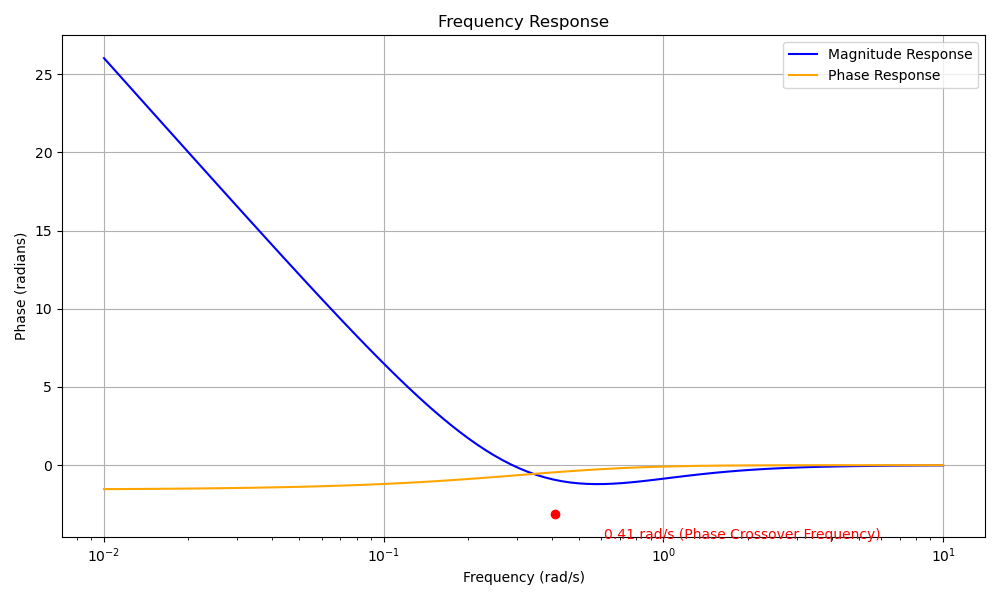
\includegraphics[width=2\columnwidth]{2023/EC/25/figs/graph.png}
\label{fig:Graph1}
\end{figure}
%\end{document}

\newpage

\item Which one of the options given is the inverse Laplace transform of $\frac{1}{s^3-s}$?\\
$u(t)$ denotes the unit-step function.
\begin{enumerate}[label=(\Alph*)]
\item $\left(-1+\frac{1}{2}e^{-t}+\frac{1}{2}e^t\right)u(t)$\\
\item $\left(\frac{1}{3}e^{-t}-e^t\right)u(t)$\\
\item $\left(-1+\frac{1}{2}e^{-(t-1)}+\frac{1}{2}e^{(t-1)}\right)u(t-1)$\\
\item $\left(-1-\frac{1}{2}e^{-(t-1)}-\frac{1}{2}e^{(t-1)}\right)u(t-1)$\\
\end{enumerate}
\hfill(GATE ME 2023)\\
\solution
\iffalse
\let\negmedspace\undefined
\let\negthickspace\undefined
\documentclass[journal,12pt,twocolumn]{IEEEtran}
\usepackage{cite}
\usepackage{amsmath,amssymb,amsfonts}
\usepackage{graphicx}
\usepackage{textcomp}
\usepackage{xcolor}
\usepackage{txfonts}
\usepackage{listings}
\usepackage{enumitem}
\usepackage{mathtools}
\usepackage{gensymb}
\usepackage{comment}
\usepackage[breaklinks=true]{hyperref}
\usepackage{tkz-euclide} 
\usepackage{listings}
\usepackage{gvv}                                        
\def\inputGnumericTable{}                                 
\usepackage[latin1]{inputenc}                                
\usepackage{color}                                            
\usepackage{array}                                            
\usepackage{longtable}                                       
\usepackage{calc}                                             
\usepackage{multirow}                                         
\usepackage{hhline}                                           
\usepackage{ifthen}                                           
\usepackage{lscape}
\usepackage[export]{adjustbox}

\newtheorem{theorem}{Theorem}[section]
\newtheorem{problem}{Problem}
\newtheorem{proposition}{Proposition}[section]
\newtheorem{lemma}{Lemma}[section]
\newtheorem{corollary}[theorem]{Corollary}
\newtheorem{example}{Example}[section]
\newtheorem{definition}[problem]{Definition}
\newcommand{\BEQA}{\begin{eqnarray}}
\newcommand{\EEQA}{\end{eqnarray}}
\newcommand{\define}{\stackrel{\triangle}{=}}
\newtheorem{rem}{Remark}

\begin{document}
\parindent 0px
\bibliographystyle{IEEEtran}

\vspace{3cm}

\title{}
\author{EE23BTECH11042 -  Khusinadha Naik$^{*}$
}
\maketitle
\newpage
\bigskip

% \renewcommand{\thefigure}{\theenumi}
% \renewcommand{\thetable}{\theenumi}


\noindent \textbf{26.} \hspace{2pt}A causal, discrete time system is described by the difference equation $y[n] = 0.5 y[n-1] + x[n]$, for all $n$, where $y[n]$ denotes the output sequence and $x[n]$ denotes the input sequence. Which of the following statements is/are TRUE?
\begin{flushright}
\hfill(GATE 2023 BM)
\end{flushright}
\begin{enumerate}[label = (\alph*)]
	\item The system has an impulse response described by $0.5^{n} u[-n]$ where $u[n]$ is the  
unit step sequence. 	\label{option:GATE.2023.BM.26.1}	
	\item The system is stable in the bounded input, bounded output sense.		\label{option:GATE.2023.BM.26.2}
	\item The system has an infinite number of non-zero samples in its impulse response	\label{option:GATE.2023.BM.26.3}
	\item The system has a finite number of non-zero samples in its impulse response.	\label{option:GATE.2023.BM.26.4}
\end{enumerate}

\noindent \textbf{Ans.}\\
\fi
\begin{table}[h]
\centering
\begin{tabular}{|c|c|c|}
        \hline
        \textbf{Parameter} & \textbf{Value} & \textbf{Description} \\
        \hline
        $x[n]$ & ? & Input Sequence \\
        \hline
        $y[n]$ & ? & Output Sequence \\
        \hline
\end{tabular}
\caption{Input parameters table}
\label{tab:GATE.2023.BM.26.1}





\end{table}
\begin{align}
y[n] = 0.5y[n-1] + x[n] 
\end{align}

Taking $Z$-Transform 
\begin{align}
Y\brak{z} &= 0.5z^{-1}Y\brak{z} + X\brak{z} \\
\implies \frac{Y\brak{z}}{X\brak{z}} &= \frac{1}{1 - 0.5z^{-1}} = H\brak{z} 
\end{align}
If $x[n]$ is impulse input 
\begin{align}
\implies &Y\brak{z} = H\brak{z} = \frac{1}{1 - 0.5z^{-1}}  \label{eq:GATE.2023.BM.26.4}
\end{align}
From \eqref{eq:GATE.2023.BM.26.4} pole lies at $z = 0.5$
\begin{align}
a^{n}u\brak{n} \xleftrightarrow{\mathcal{Z}} &\frac{1}{1 - az^{-1}} \quad , \abs{z} > a \label{eq:GATE.2023.BM.26.5}
\end{align}

From \eqref{eq:GATE.2023.BM.26.4} , \eqref{eq:GATE.2023.BM.26.5}
\begin{align}
h[n] = 0.5^{n}u[n] \quad , \abs{z} > 0.5 \label{eq:GATE.2023.BM.26.6}
\end{align}


\pagebreak
Plotting $h[n]$ vs $n$
\begin{figure}[h]
    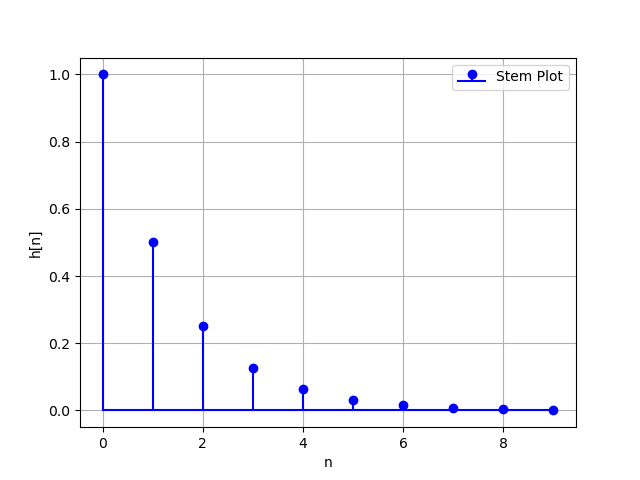
\includegraphics[width=0.5\textwidth]{2023/BM/26/figs/fig1.png}
    \caption{Plot of $h[n]$ vs $n$}
    \label{fig:GATE.2023.BM.26.1}
\end{figure}

\begin{enumerate}
\item From \eqref{eq:GATE.2023.BM.26.6} , \ref{option:GATE.2023.BM.26.1} is wrong
\item As pole lies within unit circle \ref{option:GATE.2023.BM.26.2} is true
\item From \eqref{eq:GATE.2023.BM.26.6} and \figref{fig:GATE.2023.BM.26.1} ,\ref{option:GATE.2023.BM.26.3} is true and hence
\item \ref{option:GATE.2023.BM.26.4} is false 
\end{enumerate}





%\end{document}

\newpage

\item The state equation of a second order system is \\
$ \dot{{x}}(t) = A{x}(t)$, \quad ${x}(0)$ is the initial condition. \\
Suppose $\lambda_1$ and $\lambda_2$ are two distinct eigenvalues of $A$, and $\nu_1$ and $\nu_2$ are the corresponding eigenvectors. For constants $\alpha_1$ and $\alpha_2$, the solution, ${x}(t)$, of the state equation is \\
\begin{enumerate}[label=(\Alph*)]
\item $\sum_{i=1}^{2} \alpha_ie^{\lambda_it}\bf{\nu}_i$
\item $\sum_{i=1}^{2} \alpha_ie^{2\lambda_it}\bf{\nu}_i$
\item $\sum_{i=1}^{2} \alpha_ie^{3\lambda_it}\bf{\nu}_i$
\item $\sum_{i=1}^{2} \alpha_ie^{4\lambda_it}\bf{\nu}_i$
\end{enumerate}
\hfill{GATE EC 2023}\\
\solution
\iffalse
\let\negmedspace\undefined
\let\negthickspace\undefined
\documentclass[journal,12pt,twocolumn]{IEEEtran}
\usepackage{cite}
\usepackage{amsmath,amssymb,amsfonts}
\usepackage{graphicx}
\usepackage{textcomp}
\usepackage{xcolor}
\usepackage{txfonts}
\usepackage{listings}
\usepackage{enumitem}
\usepackage{mathtools}
\usepackage{gensymb}
\usepackage{comment}
\usepackage[breaklinks=true]{hyperref}
\usepackage{tkz-euclide} 
\usepackage{listings}
\usepackage{gvv}                                        
\def\inputGnumericTable{}                                 
\usepackage[latin1]{inputenc}                                
\usepackage{color}                                            
\usepackage{array}                                            
\usepackage{longtable}                                       
\usepackage{calc}                                             
\usepackage{multirow}                                         
\usepackage{hhline}                                           
\usepackage{ifthen}                                           
\usepackage{lscape}
\usepackage[export]{adjustbox}

\newtheorem{theorem}{Theorem}[section]
\newtheorem{problem}{Problem}
\newtheorem{proposition}{Proposition}[section]
\newtheorem{lemma}{Lemma}[section]
\newtheorem{corollary}[theorem]{Corollary}
\newtheorem{example}{Example}[section]
\newtheorem{definition}[problem]{Definition}
\newcommand{\BEQA}{\begin{eqnarray}}
\newcommand{\EEQA}{\end{eqnarray}}
\newcommand{\define}{\stackrel{\triangle}{=}}
\newtheorem{rem}{Remark}

\begin{document}
\parindent 0px
\bibliographystyle{IEEEtran}

\vspace{3cm}

\title{}
\author{EE23BTECH11042 -  Khusinadha Naik$^{*}$
}
\maketitle
\newpage
\bigskip

% \renewcommand{\thefigure}{\theenumi}
% \renewcommand{\thetable}{\theenumi}


\noindent \textbf{26.} \hspace{2pt}A causal, discrete time system is described by the difference equation $y[n] = 0.5 y[n-1] + x[n]$, for all $n$, where $y[n]$ denotes the output sequence and $x[n]$ denotes the input sequence. Which of the following statements is/are TRUE?
\begin{flushright}
\hfill(GATE 2023 BM)
\end{flushright}
\begin{enumerate}[label = (\alph*)]
	\item The system has an impulse response described by $0.5^{n} u[-n]$ where $u[n]$ is the  
unit step sequence. 	\label{option:GATE.2023.BM.26.1}	
	\item The system is stable in the bounded input, bounded output sense.		\label{option:GATE.2023.BM.26.2}
	\item The system has an infinite number of non-zero samples in its impulse response	\label{option:GATE.2023.BM.26.3}
	\item The system has a finite number of non-zero samples in its impulse response.	\label{option:GATE.2023.BM.26.4}
\end{enumerate}

\noindent \textbf{Ans.}\\
\fi
\begin{table}[h]
\centering
\begin{tabular}{|c|c|c|}
        \hline
        \textbf{Parameter} & \textbf{Value} & \textbf{Description} \\
        \hline
        $x[n]$ & ? & Input Sequence \\
        \hline
        $y[n]$ & ? & Output Sequence \\
        \hline
\end{tabular}
\caption{Input parameters table}
\label{tab:GATE.2023.BM.26.1}





\end{table}
\begin{align}
y[n] = 0.5y[n-1] + x[n] 
\end{align}

Taking $Z$-Transform 
\begin{align}
Y\brak{z} &= 0.5z^{-1}Y\brak{z} + X\brak{z} \\
\implies \frac{Y\brak{z}}{X\brak{z}} &= \frac{1}{1 - 0.5z^{-1}} = H\brak{z} 
\end{align}
If $x[n]$ is impulse input 
\begin{align}
\implies &Y\brak{z} = H\brak{z} = \frac{1}{1 - 0.5z^{-1}}  \label{eq:GATE.2023.BM.26.4}
\end{align}
From \eqref{eq:GATE.2023.BM.26.4} pole lies at $z = 0.5$
\begin{align}
a^{n}u\brak{n} \xleftrightarrow{\mathcal{Z}} &\frac{1}{1 - az^{-1}} \quad , \abs{z} > a \label{eq:GATE.2023.BM.26.5}
\end{align}

From \eqref{eq:GATE.2023.BM.26.4} , \eqref{eq:GATE.2023.BM.26.5}
\begin{align}
h[n] = 0.5^{n}u[n] \quad , \abs{z} > 0.5 \label{eq:GATE.2023.BM.26.6}
\end{align}


\pagebreak
Plotting $h[n]$ vs $n$
\begin{figure}[h]
    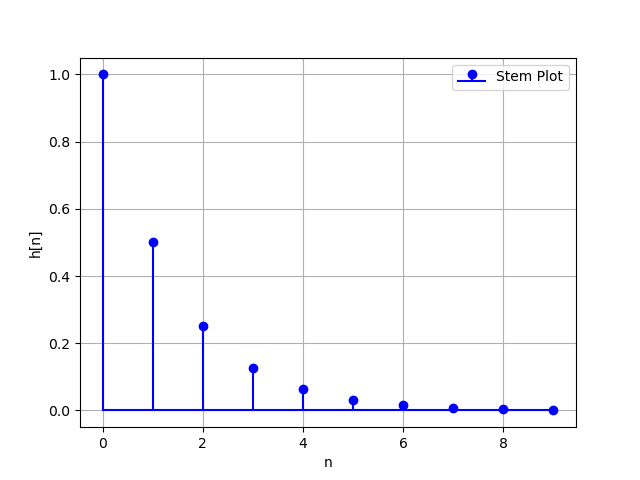
\includegraphics[width=0.5\textwidth]{2023/BM/26/figs/fig1.png}
    \caption{Plot of $h[n]$ vs $n$}
    \label{fig:GATE.2023.BM.26.1}
\end{figure}

\begin{enumerate}
\item From \eqref{eq:GATE.2023.BM.26.6} , \ref{option:GATE.2023.BM.26.1} is wrong
\item As pole lies within unit circle \ref{option:GATE.2023.BM.26.2} is true
\item From \eqref{eq:GATE.2023.BM.26.6} and \figref{fig:GATE.2023.BM.26.1} ,\ref{option:GATE.2023.BM.26.3} is true and hence
\item \ref{option:GATE.2023.BM.26.4} is false 
\end{enumerate}





%\end{document}

\newpage

\item The continuous time signal $x\brak{t}$ is described by:
\begin{align}
x\brak{t}=
    \begin{cases}
        1, & \text{if } 0\: {\displaystyle \leq }\:t\:{\displaystyle \leq }\:1\\
        0, & \text{elsewhere}
    \end{cases} 
\end{align}
If $y\brak{t}$ represents $x\brak{t}$ convolved with itself, which of the following options is/are TRUE?
\begin{enumerate}[label = (\Alph*)]
    \item $y\brak{t}$ = 0 for all $t<0$ \label{gate.bm.49.a}\\
    \item $y\brak{t}$ = 0 for all $t>1$ \label{gate.bm.49.b}\\
    \item $y\brak{t}$ = 0 for all $t>3$ \label{gate.bm.49.c}\\
    \item $\int_{0.1}^{0.75} \frac{dy\brak{t}}{dt}\: \text{dt} \neq 0$ \label{gate.bm.49.d}
\end{enumerate} \hfill{GATE 2023 BM- Q 49}\\
\input{2023/BM/49/gate.bm.49.tex}
\newpage

\item For the signals x\brak{t} and y\brak{t} shown in the figure, $z\brak{t}=x\brak{t}*y\brak{t}$ is maximum at $t=T_1$. Then $T_1$ in seconds is .......... \brak{\text{Round off to the nearest integer}}\\
\begin{tikzpicture}
\begin{axis}[xmin=-3, xmax=7, ymin=-3, ymax=3, axis lines=middle, xlabel={$t$}, title={$y\brak{t}$}]
 \addplot[blue] coordinates {(-3,0) (1,0)};
  \addplot[blue] coordinates {(1,0) (1,-2)};
   \addplot[dashed] coordinates {(0,-2) (1,-2)};
  \addplot[blue, domain=1:5] {x - 3};
  \addplot[blue] coordinates {(5,2) (5,0)};
  \addplot[blue] coordinates {(5,0) (7,0)};
  \addplot[dashed] coordinates {(0,2) (5,2)};
    \end{axis}
\end{tikzpicture}

\begin{tikzpicture}
    \begin{axis}[xmin=-3, xmax=3, ymin=-3, ymax=3, axis lines=middle, xlabel={$t$} ,title={$x\brak{t}$}]
        \addplot[blue] coordinates {(-3,0) (-1,0)};
        \addplot[blue] coordinates {(-1,0) (-1,1)};
        \addplot[blue] coordinates {(-1,1) (1,1)};
        \addplot[blue] coordinates {(1,1) (1,0)};
        \addplot[blue] coordinates {(1,0) (3,0)};
    \end{axis}
\end{tikzpicture}

\hfill (GATE EE 2023 Q 31)
\solution
\iffalse
\let\negmedspace\undefined
\let\negthickspace\undefined
\documentclass[a4,12pt,twocolumn]{IEEEtran}
%\documentclass[conference]{IEEEtran}
%\IEEEoverridecommandlockouts
% The preceding line is only needed to identify funding in the first footnote. If that is unneeded, please comment it out.
\usepackage{cite}
\usepackage{amsmath,amssymb,amsfonts,amsthm}
\usepackage{algorithmic}
\usepackage{graphicx}
\usepackage{textcomp}
\usepackage{xcolor}
\usepackage{txfonts}
\usepackage{listings}
\usepackage{enumitem}
\usepackage{mathtools}
\usepackage{gensymb}
\usepackage[breaklinks=true]{hyperref}
\usepackage{tkz-euclide} % loads  TikZ and tkz-base
\usepackage{listings}
\usepackage{empheq}
\usepackage[utf8]{inputenc}
\usepackage{pgfplots}
\usepackage{mathrsfs}
\usepackage{multicol}
\usepackage{array}
%\usepackage{setspace}
%\usepackage{gensymb}
%\doublespacing
%\singlespacing

%\usepackage{graphicx}

\DeclareMathOperator*{\Res}{Res}
%\renewcommand{\baselinestretch}{2}
\renewcommand\thesection{\arabic{section}}
\renewcommand\thesubsection{\thesection.\arabic{subsection}}
\renewcommand\thesubsubsection{\thesubsection.\arabic{subsubsection}}

\renewcommand\thesectiondis{\arabic{section}}
\renewcommand\thesubsectiondis{\thesectiondis.\arabic{subsection}}
\renewcommand\thesubsubsectiondis{\thesubsectiondis.\arabic{subsubsection}}

% correct bad hyphenation here
\hyphenation{op-tical net-works semi-conduc-tor}
\def\inputGnumericTable{}                                 %%

\lstset{
%language=C,
frame=single, 
breaklines=true,
columns=fullflexible
}
%\lstset{
%language=tex,
%frame=single, 
%breaklines=true
%}

\begin{document}
%


\newtheorem{theorem}{Theorem}[section]
\newtheorem{problem}{Problem}
\newtheorem{proposition}{Proposition}[section]
\newtheorem{lemma}{Lemma}[section]
\newtheorem{corollary}[theorem]{Corollary}
\newtheorem{example}{Example}[section]
\newtheorem{definition}[problem]{Definition}
%\newtheorem{thm}{Theorem}[section] 
%\newtheorem{defn}[thm]{Definition}
%\newtheorem{algorithm}{Algorithm}[section]
%\newtheorem{cor}{Corollary}
\newcommand{\BEQA}{\begin{eqnarray}}
\newcommand{\EEQA}{\end{eqnarray}}
\newcommand{\define}{\stackrel{\triangle}{=}}

\bibliographystyle{IEEEtran}
%\bibliographystyle{ieeetr}


\providecommand{\mbf}{\mathbf}
\providecommand{\pr}[1]{\ensuremath{\Pr\left(#1\right)}}
\providecommand{\qfunc}[1]{\ensuremath{Q\left(#1\right)}}
\providecommand{\sbrak}[1]{\ensuremath{{}\left[#1\right]}}
\providecommand{\lsbrak}[1]{\ensuremath{{}\left[#1\right.}}
\providecommand{\rsbrak}[1]{\ensuremath{{}\left.#1\right]}}
\providecommand{\brak}[1]{\ensuremath{\left(#1\right)}}
\providecommand{\lbrak}[1]{\ensuremath{\left(#1\right.}}
\providecommand{\rbrak}[1]{\ensuremath{\left.#1\right)}}
\providecommand{\cbrak}[1]{\ensuremath{\left\{#1\right\}}}
\providecommand{\lcbrak}[1]{\ensuremath{\left\{#1\right.}}
\providecommand{\rcbrak}[1]{\ensuremath{\left.#1\right\}}}
\theoremstyle{remark}
\newtheorem{rem}{Remark}
\newcommand{\sgn}{\mathop{\mathrm{sgn}}}
%\providecommand{\abs}[1]{\left\vert#1\right\vert}
\providecommand{\res}[1]{\Res\displaylimits_{#1}} 
%\providecommand{\norm}[1]{\left\lVert#1\right\rVert}
%\providecommand{\norm}[1]{\lVert#1\rVert}
\providecommand{\mtx}[1]{\mathbf{#1}}
%\providecommand{\mean}[1]{E\left[ #1 \right]}
\providecommand{\fourier}{\overset{\mathcal{F}}{ \rightleftharpoons}}
%\providecommand{\hilbert}{\overset{\mathcal{H}}{ \rightleftharpoons}}
\providecommand{\system}{\overset{\mathcal{H}}{ \longleftrightarrow}}
	%\newcommand{\solution}[2]{\textbf{Solution:}{#1}}
\newcommand{\solution}{\noindent \textbf{Solution: }}
\newcommand{\cosec}{\,\text{cosec}\,}
\providecommand{\dec}[2]{\ensuremath{\overset{#1}{\underset{#2}{\gtrless}}}}
\newcommand{\myvec}[1]{\ensuremath{\begin{pmatrix}#1\end{pmatrix}}}
\newcommand{\mydet}[1]{\ensuremath{\begin{vmatrix}#1\end{vmatrix}}}
%\numberwithin{equation}{section}
%\numberwithin{equation}{subsection}
%\numberwithin{problem}{section}
%\numberwithin{definition}{section}
%\makeatletter
%\@addtoreset{figure}{problem}
%\makeatother

%\let\StandardTheFigure\thefigure
\let\vec\mathbf

\title{
\Huge\textbf{Gate EE 2023}\\
\Huge\textbf{EE1205} Signals and Systems\\
}
\large\author{Nimal Sreekumar\\EE23BTECH11044}

% make the title area
\maketitle


%\tableofcontents

\bigskip

\renewcommand{\thefigure}{\arabic{figure}}
\renewcommand{\thetable}{\theenumi}
%\renewcommand{\theequation}{\theenumi}


\textbf{Question Gate 2023 EE:}
For the signals x\brak{t} and y\brak{t} shown in the figure, $z\brak{t}=x\brak{t}*y\brak{t}$ is maximum at $t=T_1$. Then $T_1$ in seconds is .......... \brak{\text{Round off to the nearest integer}}\\

\begin{tikzpicture}
\begin{axis}[xmin=-3, xmax=7, ymin=-3, ymax=3, axis lines=middle, xlabel={$t$}, title={$y\brak{t}$}]
 \addplot[blue] coordinates {(-3,0) (1,0)};
  \addplot[blue] coordinates {(1,0) (1,-2)};
   \addplot[dashed] coordinates {(0,-2) (1,-2)};
  \addplot[blue, domain=1:5] {x - 3};
  \addplot[blue] coordinates {(5,2) (5,0)};
  \addplot[blue] coordinates {(5,0) (7,0)};
  \addplot[dashed] coordinates {(0,2) (5,2)};
    \end{axis}
\end{tikzpicture}

\begin{tikzpicture}
    \begin{axis}[xmin=-3, xmax=3, ymin=-3, ymax=3, axis lines=middle, xlabel={$t$} ,title={$x\brak{t}$}]
        \addplot[blue] coordinates {(-3,0) (-1,0)};
        \addplot[blue] coordinates {(-1,0) (-1,1)};
        \addplot[blue] coordinates {(-1,1) (1,1)};
        \addplot[blue] coordinates {(1,1) (1,0)};
        \addplot[blue] coordinates {(1,0) (3,0)};
    \end{axis}
\end{tikzpicture}

\hfill (GATE EE 2023)
\solution
\fi

\begin{table}[htbp]
\centering
\renewcommand\thetable{1}
\begin{tabular}{|c|m{3.5cm}|m{3cm}|}
    \hline
    \textbf{Variable} & \textbf{values} & \textbf{Description} \\
    \hline
    $x\brak{t}$ & $u\brak{t+1}-u\brak{t-1}$ & signal 1\\
    \hline
    $ y\brak{t} $ & $y\brak{t} = 
    \begin{cases}
        t-3 & ; 1\leq n \leq 5 \\
        0 & ; otherwise \\
    \end{cases}$ & signal 2\\
    \hline
    $X\brak{s}$ & $\int_{0}^{\infty}x\brak{t}e^{-st}dt$ & Laplace transform of $x\brak{t}$\\
    \hline
   $Y\brak{s}$ & $\int_{0}^{\infty}y\brak{t}e^{-st}dt$ & Laplace transform of $y\brak{t}$ \\
    \hline
    $\mathscr{L^{-1}} \{Z(s)\}$ &$f\brak{t-c}u\brak{t-c}=\mathscr{L^{-1}}\brak{e^{-cs}F\brak{s}} $& Inverse Laplace transform \\
    \hline
\end{tabular}
\caption{Input Parameters}
\label{tab:11.9.5.32}
\end{table}

Using laplace transform,
\begin{align}
z\brak{t} &=x\brak{t}*y\brak{t}\label{eq:gate_ee_Q31.1} \\
Z\brak{s} &=X\brak{s}Y\brak{s}\label{eq:gate_ee_Q31.2} \\
X\brak{s} &= \frac{1}{s} \brak{e^{s}-e^{-s}} \label{eq:gate_ee_Q31.3}\\
Y\brak{s} &= \frac{2s+1}{s^2} \brak{e^{-s}-e^{-5s}}\label{eq:gate_ee_Q31.4}\\
Z\brak{s} &= \frac{2s+1}{s^3} \brak{1-e^{-4s}-e^{-2s}+e^{-6s}}\label{eq:gate_ee_Q31.5}
\end{align}
Now taking inverse laplace transform for each terms, $\mathscr{L^{-1}} \{Z(s)\}$
\begin{align}
&= \left( 2t + \frac{t^2}{2} \right) u(t) \nonumber \\
&\quad - \left( 2(t-4) + \frac{(t-4)^2}{2} \right)u(t-4) \nonumber \\
&\quad - \left( 2(t-2) + \frac{(t-2)^2}{2} \right)u(t-2) \nonumber \\
&\quad + \left( 2(t-6) + \frac{(t-6)^2}{2} \right)u(t-6) \nonumber
\end{align}\label{eq:gate_ee_Q31.6}
From the plot it is clear that $T_1=4$.\\
\begin{figure}[h]
\centering
   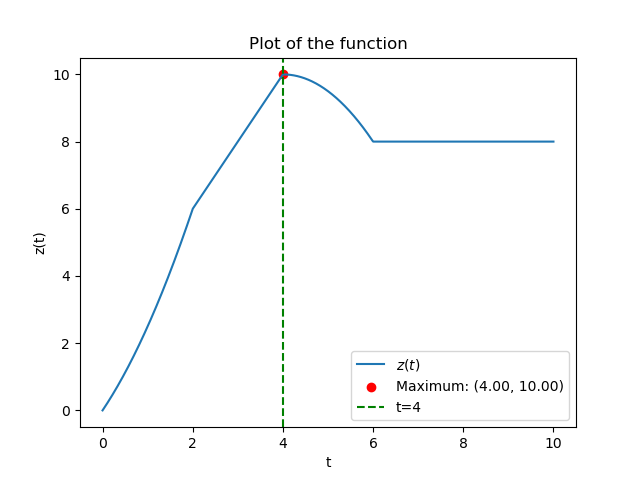
\includegraphics[width=1\linewidth]{2023/EE/31/figs/figs/gate2023EE.png}
   \caption{z\brak{t} vs. t}
   \label{fig:gate2023EE1}
 \end{figure}\\
Now in time domain,
 \begin{align}
z\brak{t} &=x\brak{t}*y\brak{t} = y\brak{t}*x\brak{t}\label{eq:gate_ee_Q31.7}\\
z\brak{t} &=\int_{-\infty}^{\infty} y\brak{\tau}x\brak{t-\tau}d\tau\label{eq:gate_ee_Q31.8}
\end{align}
$x\brak{\tau}$ is an even signal,
\begin{align}
x\brak{\tau}= x\brak{-\tau}\label{eq:gate_ee_Q31.9}\\
 x\brak{-\tau}= 
    \begin{cases}
        1 & ; -1\leq -\tau \leq 1 \\
        0 & ; \text{otherwise} \\
    \end{cases}\label{eq:gate_ee_Q31.10}
    \end{align}
    
    \begin{align}
    x\brak{-\tau} \xleftrightarrow{\text{Time shifting}} x\brak{t-\tau}\label{eq:gate_ee_Q31.11} \\
    x\brak{t-\tau}= 
    \begin{cases}
        1 & ; t-1\leq t-\tau \leq t+1 \\
        0 & ; \text{otherwise} \\
    \end{cases}\label{eq:gate_ee_Q31.12}
\end{align}\\
For $z\brak{t}$ to be maximum both $y\brak{\tau}$ and $x\brak{t-\tau}$ must be maximum,
\begin{align}
\implies t-1 &= 3 \quad \text{or} \quad t+1 = 5 \nonumber \\
t &= T_1 = 4 \nonumber
\end{align}

\newpage

\end{enumerate}
